\chapter{Flowsheet and Settings}\label{chpt.flowsheet}

This chapter provides general information about using FOQUS and constructing flowsheets. The FOQUS flowsheet provides the basis for the tools described in Chapters \ref{chpt.opt} through \ref{chpt.surrogates}. The Sections \ref{sec.flowsheet.starting.foqus} through \ref{sec.dmf} provide an overview of the FOQUS user interface, and Sections \ref{tutorial.example.files} through \ref{tutorial.fs.remote.turbine} provide tutorials.

\section{Starting FOQUS}\label{sec.flowsheet.starting.foqus}

The Windows FOQUS installer will add a FOQUS menu under ``CCSI Tools'' in the Windows start menu. Upon software installation (see the FOQUS bundle installation manual), the user can start the graphical interface using one of the following methods:
\begin{enumerate}
	\item	Select FOQUS from the Windows start menu. Note: FOQUS may be slow starting the first time, which oftentimes is related to installed anti-virus software.
	\item  Double-click a file with the ``.foqus'' extension in the Windows file explorer. FOQUS will automatically load the selected file. 
	\item	The easiest way to launch FOQUS from the command line, if it has been installed from the Windows installer, is to open ``Turbine Console'' from the FOQUS menu in the Windows start menu. The following command can be used in the command prompt:
	\begin{itemize}
		\item \texttt{foqus}
		\item \texttt{foqus --load <path to session file>}
	\end{itemize}
	The load option can take a relative or absolute path. If a relative path is specified, it is relative to the directory where the command is executed.
\end{enumerate}

The first time FOQUS is started, the user is prompted to specify a working directory. The working directory preference is stored in ``\%APPDATA\%\textbackslash.foqus.cfg'' on Windows (APPDATA is an environment variable). On Linux or OSX, the working directory is specified in ``\$HOME/.foqus.cfg''. Additionally the user can override the working directory when starting FOQUS by using the ``\texttt{--}working\_dir $\langle$working dir$\rangle$'' or ``-w $\langle$working dir$\rangle$'' command line option. Log files, user plugins, and files related to other FOQUS tools are stored in the working directory. The working directory can be changed at a later time from within FOQUS. A full list of FOQUS command line arguments is available using the ``-h'' or ``\texttt{--}help'' arguments.

\section{Session and Menu}

\subsection{Session Information Display}
%please add non-breaking space between Figure and 1 in paragraph below
Information related to a flowsheet and tool settings is organized into a FOQUS session. The session screen displays information about the current session. A menu is available by clicking the \bu{Session} drop-down menu. Figure \ref{fig.homescreen} illustrates the Home window.
\begin{figure}[H]
	\begin{center}
		\includegraphics[scale=0.55]{Chapt_flowsheet/figs/homescreen}
		\caption{Home Window}
		\label{fig.homescreen}
	\end{center}
\end{figure}
\begin{enumerate}
	\item The buttons displayed at the top of the Home window, excluding \textbf{\underline{Help}}, are tab-like buttons that change the window when selected. The depressed button indicates the currently displayed window.
	%I flipped the order of DRM-Builder and Settings in the list below based on Figure 1.  
	\begin{enumerate}
		\item \bu{Session} displays the Session window, which contains a description of the session that is currently open. \bu{Session} has a drop-down menu that displays the Session menu, which is illustrated in Figure \ref{fig.session.menu}.
		\item \bu{Flowsheet} displays the meta-flowsheet editing window.  
		\item \bu{Uncertainty} displays the interface for PSAUDE and UQ visualization.
		\item \bu{Optimization} displays the simulation-based optimization interface.
		\item \bu{OUU} displays the optimization under uncertainty interface.
		\item \bu{Surrogates} displays the surrogate model generation window.
		\item \bu{DRM-Builder} displays the dynamic reduced model builder, which can be used to develop reduced models for dynamic simulations.
		\item \bu{Settings} displays the main FOQUS settings window.
	\end{enumerate}
	\item \bu{Help} toggles the Help browser. The Help browser contains HTML help, as well as additional licensing information about other libraries and software included in the FOQUS installation.
	\item The main Session window displays information about the current session and is divided into three tabs:
	\begin{itemize}
		\item \bu{Metadata} displays information about the current FOQUS session. The \underline{\textbf{Session Name}} provides a descriptive name for the session. This name is used by the data management framework and when running flowsheets remotely, so a name is required. Entering a name should be the first step in creating a FOQUS flowsheet. \underline{\textbf{Version}} number can be used to keep track of changes to a FOQUS session. \underline{\textbf{Confidence}} describes whether the FOQUS session is expected to produce reliable results or not. \underline{\textbf{ID}} is a unique identifier to identify a particular saved version of the session. \underline{\textbf{Creation Time}} is the date and time that the flowsheet was first saved. \underline{\textbf{Modification Tim}e} is the time and date that the flowsheet was last saved. 
		\item \bu{Description} displays a detailed explanation of the purpose of the current session file, the problem being solved, and other useful information provided by the creator of the session file.
		\item \bu{Change Log} displays a record of changes made to the file. If the \textbf{\textbf{Automatically create backup session file, when saving changes}} checkbox is selected in FOQUS \textbf{\underline{Settings}}, a backup file should exist for entries in the \underline{\textbf{Change Log}}. The backup can be matched to the \underline{\textbf{Change Log}} by the unique identifier appended to the file name.
	\end{itemize}
\end{enumerate}

\subsection{Session Menu}
\label{session-menu}

Figure \ref{fig.session.menu} illustrates the \textbf{\underline{Session}} menu displayed with the data management framework (DMF) features disabled. When using the DMF, the \bu{Open Session} and \bu{Save/Save Session As} options include using the local file system or DMF database. To learn more about DMF options, see Section \ref{sec.dmf}.
\begin{figure}[H]
	\begin{center}
		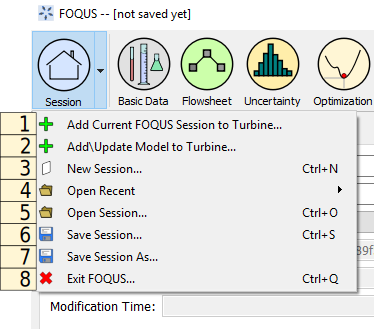
\includegraphics[scale=0.55]{Chapt_flowsheet/figs/sessionMenu}
		\caption{Home Window, Session Drop-Down Menu}
		\label{fig.session.menu}
	\end{center}
\end{figure}

The menu items in Figure \ref{fig.session.menu} are:
\begin{enumerate}
	\item \bu{Add\bs Update Model to Turbine} enables additional models to be uploaded to Turbine. Turbine provides simulation job queuing functionality so models cannot be run in FOQUS until they have been added to the Turbine server.
	\item \bu{Add\bs Update Model to DMF} enables additional models to be uploaded to the DMF. If models are uploaded to the DMF FOQUS can automatically upload the models to Turbine as needed. 
	\item \bu{New Session} clears all session information so that a new session can be started.
	\item \bu{Open Recent} shows a list of recently open FOQUS sessions that can be quickly reloaded for convenience.
	\item \bu{Open Session} opens a session that was previously saved to a file.
	\item \bu{Save Session} saves the current session with the current session file name. If the session has not been previously saved, the user will be prompted to enter a file name. \textbf{\underline{Save Session}} commands the user to save two session files: (1) a file with the selected name and (2) if backup option is enabled, a backup file with a name constructed from the \bu{Session Name} and \bu{ID}.  The Session \bu{ID} is shown on the \bu{Session, Metadata} tab.  The backup file is saved to the working directory. This system prevents accidental saving over an important file. It also enables the user to open any previously saved session.
	\item \bu{Save Session As} is similar to \textbf{\underline{Save Session}}; however, the user is prompted for a new file name.
	\item \bu{Logout from DMF Repositories} Allows the user to logout of a DMF server.
	\item \bu{Exit FOQUS} exits FOQUS. The user is asked whether to save the current session before exiting.
\end{enumerate}

\subsection{Adding or Changing Turbine Simulations}\label{overview.turbine.upload}

Before running any flowsheet where a node is linked to a simulation, the simulation must be uploaded to the Turbine gateway. To use a simulation at least two things are required: (1) the simulation file (e.g., Aspen Plus file, Excel file) and (2) the SimSinter configuration. The SimSinter configuration file is a JavaScript Object Notation (JSON) formatted file that specifies the simulation, input, and output. Any additional files required to run the simulation must also be uploaded.

Figure \ref{fig.turbine.upload} illustrates the dialog box for uploading a simulation to Turbine.
\begin{figure}[H]
	\begin{center}
		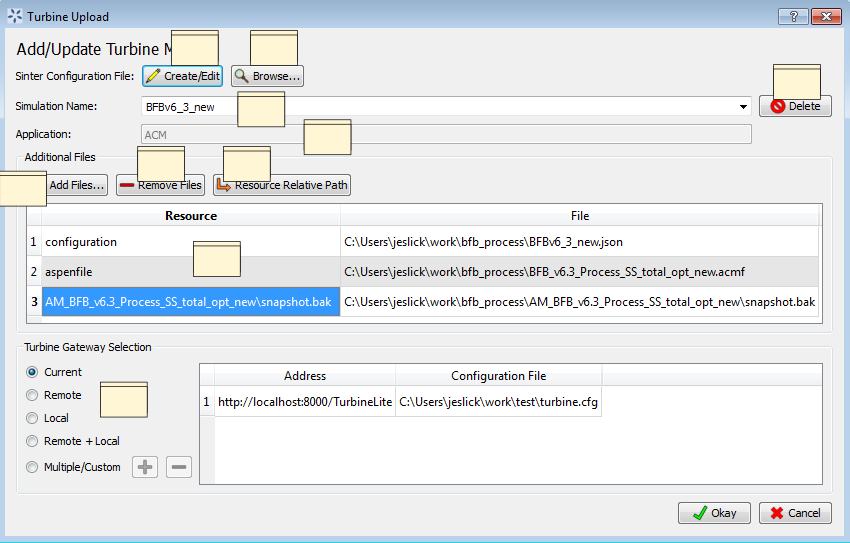
\includegraphics[scale=0.55]{Chapt_flowsheet/figs/turbineUpload}
		\caption{Turbine Upload Dialog Box}
		\label{fig.turbine.upload}
	\end{center}
\end{figure}
\begin{enumerate}
	\item \bu{Create/Edit} enables use of the SimSinter configuration Graphical User Interface (GUI) to create a SimSinter configuration file. See Chapter \ref{chapt.simsinter} and the SimSinter documentation for more information.
	\item \bu{Browse} displays a file browser, which can be used to select an existing SimSinter configuration file. Once a SimSinter configuration file is selected, the \bu{Application} type is filled in. The SimSinter \bu{Configuration File} and simulation file are automatically added to the file upload table.
	\item \bu{Simulation Name} enables entry of a new name if uploading a new simulation. An existing simulation can be selected from the drop-down list if an existing simulation is being modified. After selecting a SimSinter configuration file, the simulation name is guessed from the SimSinter configuration file name, but it can be edited.
	\item \bu{Application} displays the application that will be used to run the simulation. This is filled in automatically based on information in the SimSinter configuration file, and cannot be edited.
	\item \bu{Add Files} enables uploading of any auxiliary files that may be required by the simulation. Multiple files may be selected at once.
	\item \bu{Remove Files} enables added files to be removed from the list of files to upload.
	\item \bu{File Table} displays a list of files to be uploaded to Turbine.
	\item \bu{Delete} allows the simulation with the name currently displayed in the \bu{Simulation Name} drop-down list to be deleted from Turbine. Only simulations that have not been run can be deleted.
	\item \bu{Resource Relative Path} enables the user to set the path of resource files relative to the simulation working directory. To set the directory, select files in the \bu{File Table}. Multiple files can be selected. Click \bu{Resource Relative Path}, and type the relative path to assign to the selected resource files.
	\item \bu{Turbine Gateway Selection} enables the user to select the instance of Turbine to which to upload the simulation. \bu{Current} is the Turbine instance currently set to run simulations. \bu{Remote} is configured Remote instance. \bu{Local} is the TurbineLite instance installed on the local computer. \bu{Remote + Local} allows simulations to be uploaded to both the local and remote instances of Turbine. \bu{Multiple/Custom}  allows simulations to be uploaded to other Turbine instances by selecting Turbine configuration files.
\end{enumerate}

\subsection{Adding or Changing Data Management Framework  Simulations}\label{overview.dmf.upload}

\textbf{Please see Section \ref{sec.dmf} for information about setting up the data management framework (DMF) for use with FOQUS.}

The DMF allows storing and tracking changes for simulations.  Simulations from the DMF can be used in the FOQUS flowsheet, and FOQUS will automatically upload the simulations to Turbine as needed. The procedure for adding and updating simulations in the DMF is similar to uploading to Turbine, described in Section \ref{overview.turbine.upload}.  

The upload to DMF dialog is shown below in Figure \ref{fig.dmf.upload}. To change between the local DMF lite and DMF server, use the \bu{SelectDMF} button (see item 1 in Figure \ref{fig.dmf.upload}). For more information see Section \ref{overview.turbine.upload} and \ref{sec.dmf}.

\begin{figure}[H]
	\begin{center}
		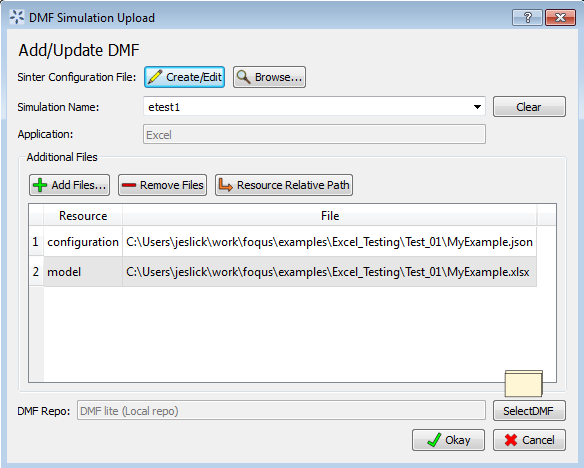
\includegraphics[scale=0.55]{Chapt_flowsheet/figs/dmfUpload}
		\caption{DMF Upload Dialog Box}
		\label{fig.dmf.upload}
	\end{center}
\end{figure}



\section{Settings}
\label{section.settings}

The settings screen shows FOQUS settings that are related to the general FOQUS setup, and are unlikely to change between sessions. The settings screen is accessible by clicking the \bu{Settings} button at the top of the Home window. The FOQUS settings can be stored in two locations: (1) ``\%APPDATA\%\bs.foqus.cfg'' on Windows or ``\$HOME/.foqus.cfg'' on Linux or OSX, (2) ``foqus.cfg'' in the working directory.

The Settings screen displays settings grouped into tabs. Figure \ref{fig.settings.options} shows \bu{Settings, FOQUS} tab. 

\begin{figure}[H]
	\begin{center}
		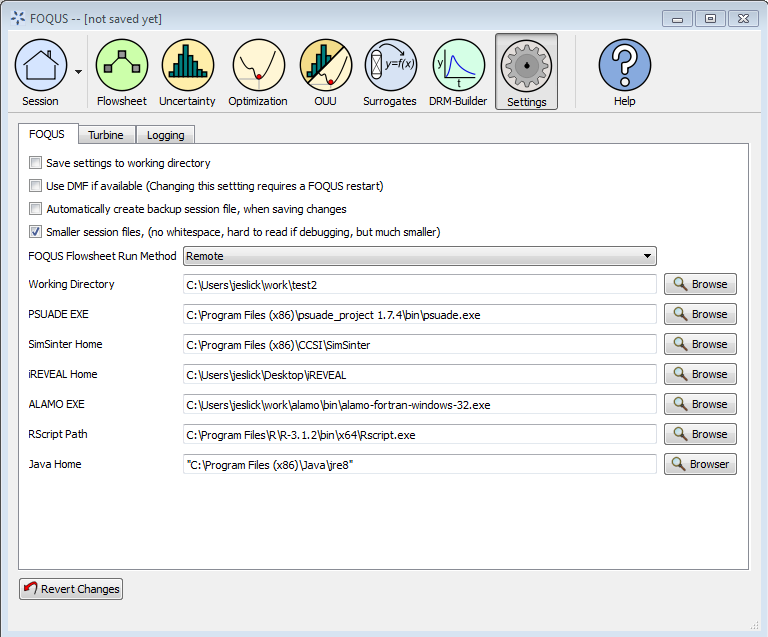
\includegraphics[scale=0.55]{Chapt_flowsheet/figs/settings_options}
		\caption{Settings, FOQUS Tab}
		\label{fig.settings.options}
	\end{center}
\end{figure}

Options in the \bu{Settings, FOQUS} tab are described below.
\begin{enumerate}
	\item  \bu{Save settings to working directoy}, when checkbox is selected the settings file will be read from the specified working directory. This setting is useful for running multiple copies of FOQUS to ensure the settings do not conflict. When starting additional copies of FOQUS, it is best to start them from the Working Directory command line giving each copy of FOQUS its own independent working directory. If FOQUS is started more than once from the Windows start menu, each copy will use the same working directory. Starting FOQUS multiple times with the same working directory may cause unusual behavior in FOQUS.
	\item \bu{Use DMF if available}, when checkbox is selected the Data Management Framework (DMF) module will be loaded and the DMF options will be shown in the \textbf{Session\underline{}} menu.
	\item \bu{Automatically create backup session file}, when checkbox is selected each time a FOQUS session is saved it will be saved twice. A backup copy with a universally unique identifier appended to the file name will be saved.  This will allow the user to load any previous save point of the session.
	\item \bu{Smaller session files}, when checkbox is selected significant storage space is saved by excluding formatting from the session file; this makes the session files less human readable. A more readable session file can be useful for debugging.
	\item \bu{FOQUS Flowsheet Run Method} enables the user to select between running simulations on the same computer as FOQUS, or on a remote Turbine gateway. Running simulations remotely allows parallel execution. The default setting is "Local". If the user switches from "Local" to "Remote", a warning message will appear. The user will be informed that the models that have been uploaded to the Local Turbine may not be available in the Remote Turbine Gateway. Therefore, the user may need to upload these models into Turbine again in order to run the models remotely.
	%Please fix the margins in the paragraph below - Working Directory in the paragraph is displaying beyond the right margin. 
	\item \bu{Working Directory} is the path to the FOQUS working directory. The \textbf{\underline{Working Directory}} is where FOQUS reads and writes files needed to function. When running multiple copies of FOQUS, the \textbf{\underline{Working Directory}} can also be specified from the command line using the ``-w'' or ``--workingDir'' options. After changing the \textbf{\underline{Working Directory}}, FOQUS should be restarted.
	\item \bu{PSUADE EXE} is the path to the PSUADE executable. PSUADE provides FOQUS's UQ features.
	\item \bu{SimSinter Home} is the path to the SimSinter interface for creating Sinter configuration files for simulations to be run with FOQUS. This setting is not required but it allows easy access to the SimSinter configuration GUI when uploading simulation to Turbine.
	\item \bu{iREVEAL Home} is the path the iREVEAL installation. This is required to use the iREVEAL surrogate model module.
	\item \bu{ALAMO EXE} is the path to the ALAMO executable. This is required to use the ALAMO surrogate model module.
	\item \bu{RScript Path} is the path to the RScript executable. This is required for surrogate model modules that use R as a platform.
	\item \bu{Java Home} is the path to the Java installation. The DMF and the iREVEAL surrogate modules require Java.
	\item \bu{Revert Changes} The settings changes are applied when the user navigates away from the settings screen. To undo changes made to settings the revert button can be clicked before changing to another screen.
\end{enumerate}


The \bu{Turbine} tab contains settings for configuring the local and remote instance of Turbine. Figure \ref{fig.settings.turbine} shows the FOQUS Turbine settings.

\begin{figure}[H]
	\begin{center}
		\includegraphics[scale=0.55]{Chapt_flowsheet/figs/settings_turbine}
		\caption{Settings, Turbine Tab}
		\label{fig.settings.turbine}
	\end{center}
\end{figure}

The first section in the \textbf{\underline{Turbine}} tab is \bu{TurbineLite (Local)}. This section contains settings related to the local installation of Turbine, and is only applicable when running FOQUS on the windows platform.
\begin{enumerate}
	\item \bu{Test} tests the connection to the local Turbine server to make sure it is configured and running properly.
	
	\item \bu{Start Service} starts the Turbine server service on Windows. The user must have permission to start services to use this button.
	
	\item \bu{Stop Service} stops the Turbine server service on Windows. The user must have permission to stop services to use this button.
	
	\item \bu{Change Port} can reconfigure the local Turbine server service on Windows to use a different port. This may be necessary if Turbine conflicts with another service.
	
	\item \bu{Aspen Version}, Aspen 7.3 is still in common use but the API differs slightly form newer versions. This option allows FOQUS to be used with Aspen 7.3.
	
	\item \bu{TurbineLite Home} is the location of the TurbineLite installation. For local simulation runs FOQUS needs to know where TurbineLite is installed so it can launch Turbine consumers to run simulations. This setting is not needed if simulations are only run remotely.
		
	\item \bu{Turbine Configuration (local)} is the path to the TurbineLite gateway configuration file for running simulations locally. If simulations are only run remotely, this setting is not needed. \bu{New/Edit} displays a form to create or edit a Turbine configuration file. Having a setting for both local and remote Turbine allows easy switching between run methods.
	
\end{enumerate}

The second section in the \bu{Turbine} tab is \bu{Turbine Gateway (Remote)}. This section contains settings related to a remote instance of Turbine.

\begin{enumerate}
	\item \bu{Test} tests the connection to the remote Turbine server to make sure it is configured and running properly.

	\item \bu{Turbine Configuration (remote)}, is the path to the Turbine gateway configuration file for running simulations remotely. If simulations are only run locally, this setting is not needed. \bu{New/Edit} displays a form to create or edit a Turbine configuration file. Having a setting for both local and remote Turbine allows easy switching between run methods.
	
	\item \bu{Check Interval (sec)} is the number of seconds between checking the remote Turbine server for job results. This number should not be set too low to avoid overwhelming the Turbine server with requests.
	
	\item \bu{Number of Times to Resubmit Failed Jobs} is the number of times to resubmit jobs that fail. Jobs occasionally fail due to software bugs. This allows a job to be retried.

\end{enumerate}

The \bu{Logging} tab contains settings related to the FOQUS log files, which provide debugging information. The FOQUS log files are stored in the logs directory in the working directory. Figure \ref{fig.settings.logging} show the FOQUS log settings. There are two log files (1) FOQUS and (2) Turbine Client.

\begin{figure}[H]
	\begin{center}
		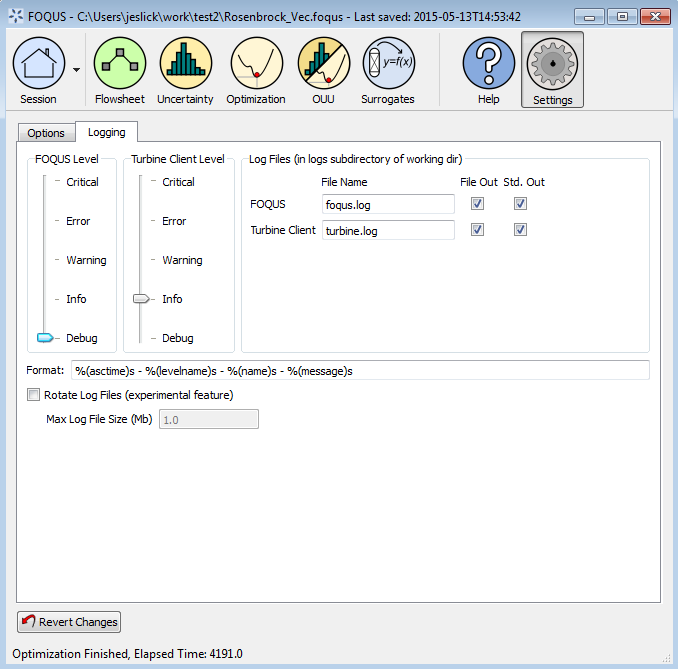
\includegraphics[scale=0.55]{Chapt_flowsheet/figs/settings_logging}
		\caption{Settings, Logging Tab}
		\label{fig.settings.logging}
	\end{center}
\end{figure}

\begin{enumerate}
	\item The level sliders indicate how much information to send to the logs.
	\item The \textbf{\underline{Log Files}} section enables the user to specify where the log information is sent. The \bu{File Out} checkboxes turn on or off the file output of logs. The \bu{Std. Out} checkboxes enable or disable the output to the screen.
	\item \bu{Format} allows the format of the log messages to be changed. See the documentation for the Python 2.7 logging module for more information.
	\item \bu{Rotate Log Files} turns on or off log file rotation. When a log file reaches a certain size, a new log file is started and the contents of the old log are moved to a new file. There currently seems to be a bug in the log file rotation which occasionally makes the log file output stop; therefore, the \bu{Rotate Log Files} option is labeled as an experimental feature.
\end{enumerate}

\section{Flowsheet}
\label{section.flowsheet}

The meta-flowsheet defines connections between simulations. The flowsheet defines the order that simulations are performed and what data is transferred between them.  Simulations are represented as nodes in the flowsheet. These simulations may be links to external simulation software through the Turbine gateway, or custom simulations or simulation wrappers written in Python. Directed edges in the flowsheet connect nodes. The edges also specify which variables in the simulations are equivalent.  

If the flowsheet contains cycles, they are solved iteratively. Tear streams are selected by FOQUS based on two criteria: (1) minimize the maximum number of times any cycle is torn and (2) minimize the total number of tear edges (which only is considered when two tear sets have the same value for the first criteria).

FOQUS currently has two methods available for solving flowsheets with recycle: (1) direct substitution and (2) Wegstien \citep{Wegstein_1958}. FOQUS will solve strongly connected components in the order they are encountered in the flowsheet. FOQUS flowsheets are generally not very complicated, so if a strongly connected component contains more than one tear stream, they are solved simultaneously.  More advanced solution options will be added if a need arises. Figure \ref{fig.flowsheet.recycle} shows how a simple flowsheet with recycle would be solved.
\begin{figure}[H]
	\begin{center}
		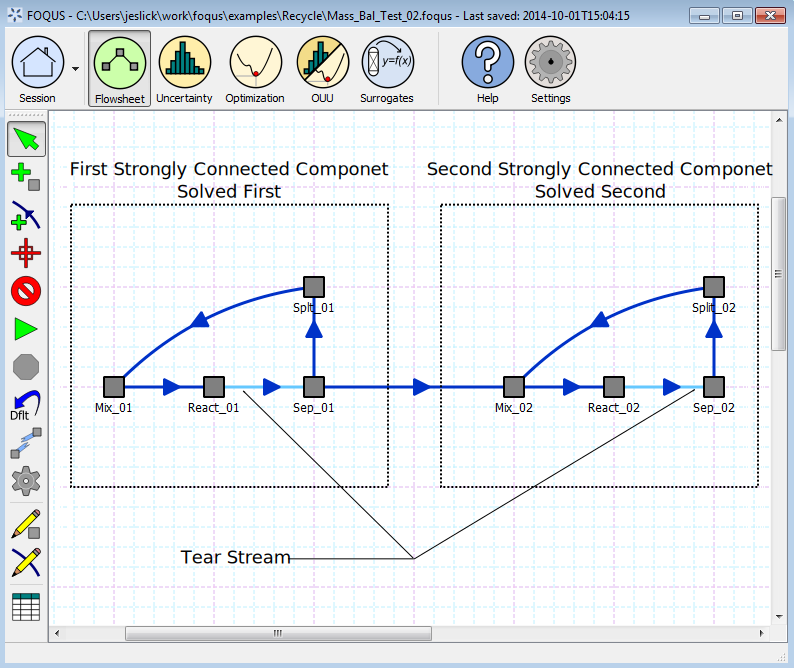
\includegraphics[scale=0.55]{Chapt_flowsheet/figs/recycle}
		\caption{Flowsheet Recycle}
		\label{fig.flowsheet.recycle}
	\end{center}
\end{figure}

\subsection{Flowsheet Editor}
Figure \ref{fig.flowsheet.editor} illustrates the main \bu{Flowsheet Editor} screen and a description of the pieces. The toolbar on the left contains various flowsheet tools.
\begin{figure}[H]
	\begin{center}
		\includegraphics[scale=0.55]{Chapt_flowsheet/figs/flowsheetEdit}
		\caption{Flowsheet Editor}
		\label{fig.flowsheet.editor}
	\end{center}
\end{figure}

The first three buttons are mouse mode buttons.  The current mouse mode is shown by the depressed button. The remaining buttons on the toolbar perform an action. The flowsheet editing toolbar and flowsheet are described in detail below.
\begin{enumerate}
	\item \bu{Selection mode} enables the user to select nodes and edges. Multiple items may be selected by holding down the Shift key. To deselect everything, click an empty area of the flowsheet while not holding the Shift key. Selected items can be moved by dragging them. To move multiple items, hold down the Shift key while dragging. The last item selected becomes the current object to be edited in the \bu{Node} or \bu{Edge Editor}.
	\item \bu{Add node mode} enables the user to add a node by clicking anywhere on the flowsheet. Once a location is clicked, a dialog box opens where the new node name can be entered. If \textbf{\underline{Cancel}} is selected, no node is added. The new node name cannot be ``graph'' and cannot match any existing node name.
	\item \bu{Add edge mode} enables edges to be added by selecting the node that the edge originates from, followed by the node the edge terminates at.
	\item \bu{Center flowsheet in display} centers the display on the flowsheet.
	\item \bu{Delete selected} deletes all selected nodes and edges. If a node is deleted, all edges connecting to that node are also deleted.
	\item \bu{Run a simulation} starts a single simulation run. This is primarily used to test a simulation before running optimization or UQ.
	\item \bu{Stop a simulation} is enabled when a simulation is running and stops any running simulation. The simulation may take several seconds to stop.
	\item \bu{Set inputs to defaults} returns all of the inputs to their default values.
	\item \bu{Determine tear edges} makes it easier to see where initial guesses are needed and makes it possible to edit the tear set before running the flowsheet.  If tear streams are needed but not specified before running a flowsheet, they will be automatically specified, however inputs that will be used for the initial guess will not be known before running.
	\item \bu{Flowsheet solver settings} contains options related to tear solvers.
	\item \bu{Toggle node editor display} displays or hides the \bu{Node Editor}. The user can change the node being edited by selecting from \bu{Name} in the \bu{Node Editor} or selecting it on the flowsheet in selection mode.
	\item \bu{Toggle edge editor display} displays or hides the edge editor. The user can change the edge being edited in the \bu{Edge Editor}, or by selecting it in selection mode.
	\item \bu{Show results from all flowsheet runs} displays the results of all flowsheet runs in a table view. This can be exported to a spreadsheet.
	\item \bu{Node} represents a simulation or calculations.
	\item \bu{Edge} connects simulation data, represents data transfer between two nodes.
\end{enumerate}

\subsection{Node Editor}
The \textbf{\underline{Node Editor}} enables the assignment of simulations to a node, and editing variables. Figure \ref{fig.node.editor.input} shows the Node Editor window with the input variables section of the toolbox displayed.
\begin{figure}[H]
	\begin{center}
		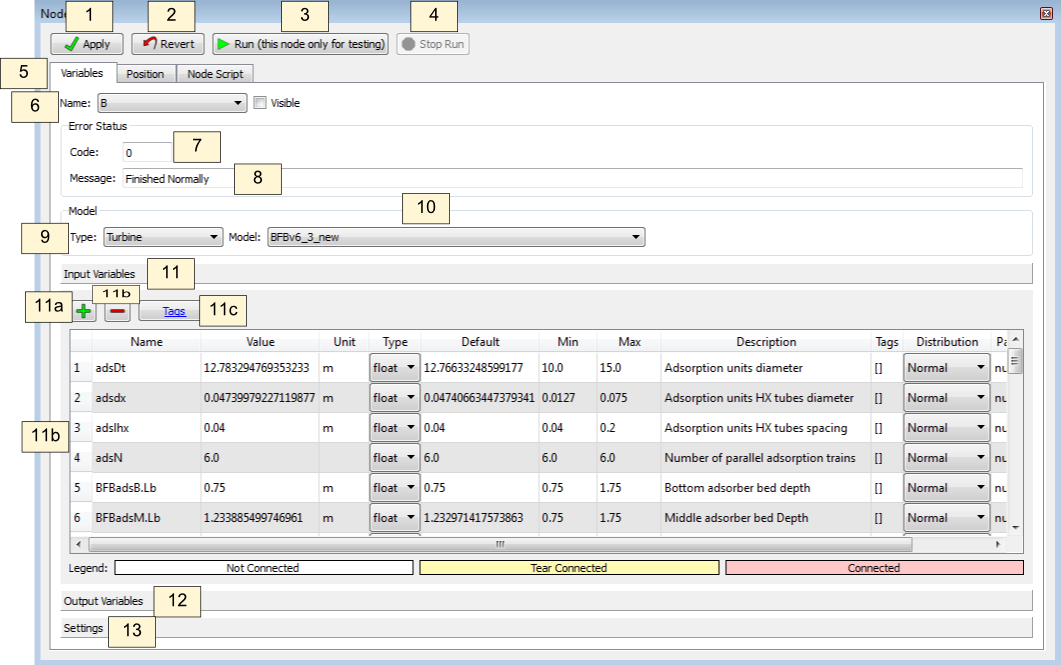
\includegraphics[scale=0.55]{Chapt_flowsheet/figs/nodeEditInput}
		\caption{Node Editor Window}
		\label{fig.node.editor.input}
	\end{center}
\end{figure}

\begin{enumerate}
	\item \bu{Apply} immediately applies any changes made in the \textbf{\underline{Node Editor}}. This is not usually needed. Changes are applied when the current node is changed, the \textbf{\underline{Node Editor}} is closed, or some other action is taken that requires the flowsheet, such as running the flowsheet.
	\item \bu{Revert} sets the node back to the version where the changes were last applied.  This is usually the original state of the node when the editor was opened.
	\item \bu{Run} can be used to run the simulation represented by this node only.  This can be used for testing to make sure the node is properly configured without running the whole flowsheet.
	\item \bu{Stop Run} is active when a simulation is currently running. It stops a single node run or a flowsheet run.
	\item There are three tabs in the \textbf{\underline{Node Editor}}: (1) \bu{Variables} tab, shown in Figure \ref{fig.node.editor.input}, (2) \bu{Position} tab displays the coordinates of the node, and (3) \bu{Node Script} tab enabling the entry of Python code to be executed after the simulation is run.
	\item \bu{Name} displays the name of the node currently being edited. The current node can be changed by selecting from existing nodes in the drop-down menu.
	\item \bu{Code} displays the error status code for the node.
	\item \bu{Message} displays a more detailed description of the error status of the node.
	\item \bu{Type} enables the user to select the type of model to run. The model types are none, Turbine, DMF Lite, DMF Server, or Python Plugin. None allows no model to be assigned to the node; this is useful when the node only executes a script entered directly into FOQUS. Turbine is used to execute Aspen, gPROMS, or Excel simulations. If simulations are stored in either the DMF lite or DMF server, the DMF type models can be used. FOQUS will automatically upload DMF models to Turbine as needed. Python plugins are custom simulations or wrappers written by the user.  Surrogate model methods may also produce Python plugin models.
	\item \bu{Model} enables selection of the models available on Turbine or loaded Python plugins.
	\item \bu{Input Variables} enables viewing and editing the node's input variables. Most of these variables are added automatically when a simulation is selected.
	\begin{enumerate}
		\item \bu{Add variable} enables the addition of an input variable. There are two reasons to add an input: (1) to use a variable to pass information to another simulation (even if the variable is not used in any node calculation, it can receive data from the previous simulation and be passed on to the next simulation) and (2) to use in a node script. For example, a variable could be added that provides output in different units of measure.
		\item \bu{Remove variable} removes variables. If an input variable is removed that originally came from a Turbine simulation, the simulation will run with the default value.
		\item \bu{Tags} displays a tag browser that lists commonly used variable tags.
		\item \bu{Input Variables} table displays information about variables. Most attributes can be edited, except for the \textbf{\underline{Name}} column within the \textbf{\underline{Input Variables}} table. The rows for input variables are color coded depending on whether they are set by an edge from results in another node. White rows are not connected. Yellow rows are set by a tear edge. These variables serve as initial guesses but their value may change once the simulation has run. Red rows are set by an edge that is not a tear edge. The value set for these inputs does not matter and it may change once the simulation has run.
	\end{enumerate}
	\item \bu{Output Variables} is a variable table similar to the \textbf{\underline{Input Variables}} table for node output variables.  This area is displayed by clicking \bu{Output Variables}.
	\item \bu{Settings} displays simulation settings. A description is provided for each setting. The available settings vary depending on simulation.
\end{enumerate}

\subsection{Node Variables}
Variables in the node editor are grouped into two sections, inputs and outputs. The input and output variable tables are accessible as described in the previous section.  The contents of the variable tables are described here.

The columns in the input variable list are:
\begin{itemize}
	\item \bu{Name} is the name of the variable,
	\item \bu{Value} is the current value,
	\item \bu{Unit} is the unit of measure,
	\item \bu{Type} is the data type (float, int, or str),
	\item \bu{Default} is the default value,
	\item \bu{Min} is the minimum value,
	\item \bu{Max} is the maximum value,
	\item \bu{Description} is a description string,
	\item \bu{Tag} is a list of strings that can be used to attach additional information to a variable
	\item \bu{Distribution} is a distribution type,
	\item \bu{Param1} is the first parameter of a parametric distribution the exact meaning depends on the selected distribution, and
	\item \bu{Param2} is the second parameter of a parametric distribution the exact meaning depends on the selected distribution.
\end{itemize}
The minimum and maximum values for are not enforced when running simulations are not enforced.  A value can be given outside the range. Optimization and UQ features make use of these values to set upper and lower bounds on decision variables or sampling. The distribution information is used when setting up sampling for UQ.  In the future, this may also be used for things like optimization under uncertainty.  Integer and string type variables cannot currently be used as optimization decision variables, or sampled with the UQ tool.

The rows of the input variable table are color coded.  Some of the input variables may be set by connections to other nodes.  White rows are variables who's values are not set by a connection.  The variables that are red have values set by a connection, and the value given will be overwritten and does not matter.  The values that are colored yellow are inputs set by a connection that is a tear stream.  The values of these variables serves as an initial guess for solving recycles.

The output variable table is similar to the input table, however it only contains the columns: Name, Value, Unit, Type, Description, and Tags.  The value of the outputs may not correspond to the inputs until the simulation has been run.


\subsection{Node Script}

There are three type of \textbf{\underline{Node Script}} that can be used: (1) \bu{Pre} runs before a node simulation, (2) \bu{Post} runs after a node simulation, and (3) \bu{Total} scripts how a node runs the simulation.

Figure \ref{fig.post.calc} illustrates the \bu{Node Script} tab of the \textbf{\underline{Node Editor}} with calculations for an optimization test problem.

\begin{figure}[H]
	\begin{center}
		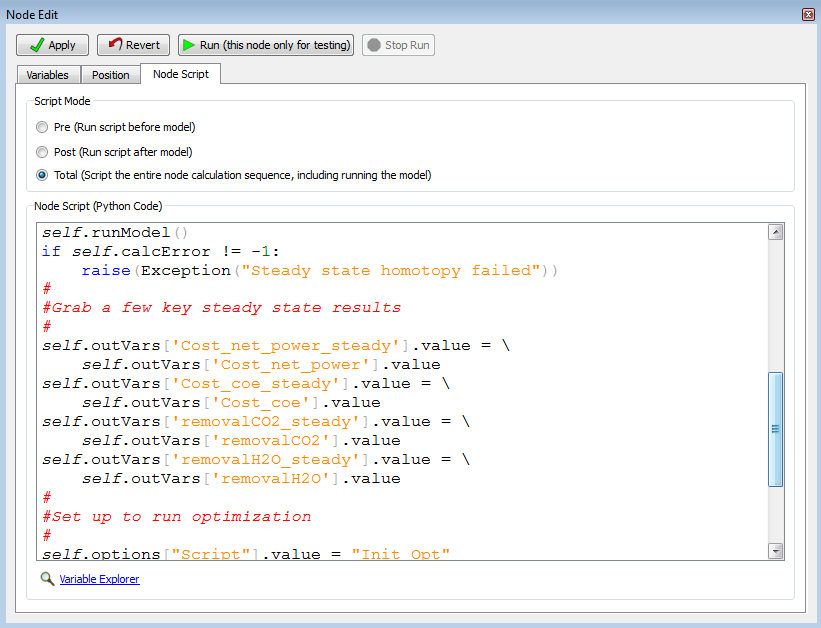
\includegraphics[scale=0.55]{Chapt_flowsheet/figs/postCalc}
		\caption{Node Script Tab}
		\label{fig.post.calc}
	\end{center}
\end{figure}

Node scripts can be any valid Python code. The input and output variables for node scripts are stored in dictionaries x and f. The dictionary keys are the variable names. The f dictionary is used to update the node variables after the calculations are executed.

\subsection{Edge Editor}
The \textbf{\underline{Edge Editor}} is illustrated in Figure \ref{fig.edge.editor}.  The \textbf{\underline{Edge Editor}} can be used to set connections between node variables.

\begin{figure}[H]
	\begin{center}
		\includegraphics[scale=0.55]{Chapt_flowsheet/figs/edgeEdit}
		\caption{Edge Editor}
		\label{fig.edge.editor}
	\end{center}
\end{figure}
\begin{enumerate}
	\item \bu{Index} is the index of the current edge. The current edge can be changed by selecting an index from the drop-down menu, but since the index is not a very meaningful identifier it is usually more convenient to select the edge to edit with the graphical selection tool.
	\item \bu{Origin Node} is the node where an edge starts. This may be edited by selecting a different node from the drop-down menu.
	\item \bu{Destination Node} is the node to which the edge goes.
	\item \bu{Curve} can be a positive or negative number. The greater the magnitude of number, the more curved an edge will appear in the flowsheet. This setting is used to keep edges from overlapping in the flowsheet display.
	\item \bu{Tear} marks this edge as a tear.  Before a simulation is run, if a valid tear set is not specified, FOQUS locates one.
	\item \bu{Active} specifies whether the edge is active or not. This allows connections to be temporarily disabled.
	\item \bu{Variable Connections} table displays which variables are connected.  Inputs or outputs in the origin node can be connected to inputs in the destination node.
	\item \bu{Add connection} adds a new connection.
	\item \bu{Remove connection} deletes the selected connections.
	\item \bu{Auto} automatically connects variables having the same name. For example, in connecting a simulation to a spreadsheet to calculate costs there are a large number of variables for which it makes sense that the variables have the same name in the simulation and spreadsheet. \bu{Auto} should be used with great care. Connecting variables with the same name is often not what is wanted. For example two simulations may have a variable named FlowAIn; however, it is very unlikely that they should be connected. It is more likely FlowAOut should be connected to FlowAIn.
\end{enumerate}


\section{Sample Results}\label{sec.flowsheet.results.table}

Flowsheet evaluations that have been run in a FOQUS session can be viewed by clicking the table button in the flowsheet toolbar (\#13 in Figure \ref{fig.flowsheet.editor}). The results are displayed in a table, and the contents can be copied and pasted into a spreadsheet or exported to a CSV file. Figure \ref{fig.results.table} show the Flowsheet Results Table window.


\begin{figure}[H]
	\begin{center}
		\includegraphics[scale=0.55]{Chapt_flowsheet/figs/resultsTable}
		\caption{Flowsheet Results Table Window}
		\label{fig.results.table}
	\end{center}
\end{figure}
\begin{samepage}
\begin{enumerate}
	\item \bu{Menu} contains a menu with four sub menus.
	\begin{enumerate}
		\item \bu{Import} data from files or the clipboard.
		\item \bu{Export} data to files or the clipboard.
		\item \bu{Edit} or delete data.
		\item \bu{View} options for the table.
	\end{enumerate}
	\item The \textbf{\underline{Current Filter}} drop-down list enables the user to select a data filter, which can be used to filter and sort data.
	\item \bu{Edit Filters} enables the user to create or edit data filters.
\end{enumerate}
\end{samepage}

\subsection{Error Codes}
Error codes are listed in the \textbf{\underline{Flowsheet Results}} table for the whole flowsheet and for individual nodes. Table \ref{table.fs.error} shows the flowsheet error codes and Table \ref{table.node.error} shows the node error codes. The most common flowsheet error is 1, a node calculation failed. The most common node error is 7, Turbine simulation error. These errors are typically caused by a simulation that fails to converge or has some other calculation error (e.g., ACM does not converge or an Excel spreadsheet simulation with a division by 0 error). 

\begin{table}[H]
	\begin{center}
		\caption{Flowsheet Error Codes}\label{table.fs.error}
		\begin{tabularx}{4.5in}{r l}
			\hline
			Code & Meaning \\
			\hline
			-1 & Did not run or finish  \\
			 0 & Success \\
			 1 & A node calculation failed \\
			 3 & Failed to create a worker node \\
			 5 & Unknown tear solver \\
			11 & Wegstein failed to converge \\
			12 & Direct failed to converge \\
			16 & Presolve node error \\
			17 & Postsolve node error \\
			19 & Unhandled exception during evaluation (see log)\\
			20 & Flowsheet thread terminated \\
			21 & Missing session name \\
			40 & Error connecting to Turbine \\
			50 & Error loading session or inputs \\
			100 & Single node calculation success \\
			201 & Cycle in determining calculation order (invalid tear set) \\
			\hline
		\end{tabularx}
	\end{center}
\end{table}

\begin{table}[H]
	\begin{center}
		\caption{Node Error Codes}\label{table.node.error}
		\begin{tabularx}{4.5in}{r l}
			\hline
			Code & Meaning \\
			\hline
			-1 & Did not run or finish  \\
			0 & Success \\
			1 & Simulation error (see log) \\
			3 & Exceeded maximum wait time \\
			4 & Failed to create Turbine session ID \\
			5 & Failed to add Turbine job \\
			6 & Exceeded maximum run time\\
			7 & Turbine simulation error \\
			8 & Failed to start Turbine job \\
		   10 & Failed to get Turbine jobs status \\
		   11 & Flowsheet thread terminated \\
		   20 & Error in node script\\
		   23 & Could not convert Numpy value to list \\
		   27 & Cannot read variable result (see log)\\
			\hline
		\end{tabularx}
	\end{center}
\end{table}
%\section{Data Management Framework (DMF)}
\label{sec.dmf}
The Data Management Framework (DMF) provides a central,
network-accessible service to archive and track all files related to a
carbon capture investigation. It facilitates group interactions by
providing a venue to share documents between multiple, geographically
distributed individuals while tracking the relationships between these
files. It is intended to store all the data related to a project from
the gathering of experimental data, to the development of basic
models, to the development of process models, and ultimately
optimization and UQ studies.

In addition to providing basic file sharing services, the DMF is setup
to store multiple revisions of each file in the system and it
provides a historical archive of the evolution of the project. Older
version of data and model files are stored to enable backtracking or
to provide a means to compare the final product with earlier work.

The DMF can also be used to track the provenance of simulation
results. As files are added to the DMF, the user specifies
relationships between individual files to indicate a dependency. For
example, a basic model file depends on a file containing experimental
data, and a process model file depends on the basic model
file. Collections of these dependency relationships help establish
the provenance chain for each file in the system. This enables DMF
users to see when dependencies of a simulation
have been modified, indicating that the simulation may not be
incorporating the best available data.

A lightweight version of the DMF (known as the DMF lite), is also now available.
The DMF lite provides fewer functionalities than its server-based counterpart.
Version control and metadata for data objects are provided in the DMF lite,
but provides no search and minimal dependency tracking functionality (only tracks
dependencies for simulations). It is designed to work locally without the
need for a centralized server.

This section discusses the various components bundled with FOQUS.
There are three main components, which enables the user to open,
save, browse, and edit files in the DMF. A separate tool for
ingesting basic data models is also bundled in FOQUS. These are discussed in
more detail in the subsections below.

\subsection{Setup for Use with FOQUS}
\label{dmf-setup}

The DMF has two modes. It can be setup to be used on the local machine (DMF lite) or with a server.
The former, DMF lite, depends on Git as its backend while the latter uses an Alfresco data repository as its backend.
Both modes can be operated independently of each other. Setup instructions for both modes are specified below.

\subsubsection{DMF Lite}
The DMF is a lightweight DMF that requires minimal dependencies and is meant to be used by a single user.
In the case of the DMF lite, the Git distributed version control system is all that needs to be installed.
The DMF lite
was developed with Git version 2.5.0, but should work with newer versions as well. When
installing Git on Windows, the options (1) Use Git from the Windows Command Prompt and
(2) Checkout as-is, commit Unix-style line endings should be selected.

Certain features in the DMF lite are meant to be synced with a server. If these features are desired,
instructions in the following subsection will be needed.

\subsubsection{DMF (with Server)}
\label{dmf-with-server}
To enable FOQUS to access the server-based DMF, the following steps are needed:
\begin{enumerate}
\item Creation of properties file.
\item Execution of build script.
\item Installation of certificates (Note: This is only needed if server uses the https protocol.)
\end{enumerate}
Each step is independent and does not need to be executed in order. More details are provided below.

\textbf{Properties file:}
For each server-based DMF, a
.properties file (files that have .properties as an extension) must first be created. Multiple
.properties files can be added to enable access to multiple servers.
These files provide the configuration information that
is needed for FOQUS to locate one or more DMF repositories.
(\textbf{Important:} It is important that the file ends with the .properties extension. The fields
specified in the .properties file are also case-sensitive.)

For Windows systems, these files must be placed under the ``\%APPDATA\%'' directory.
For Linux or OS X systems, the files must be placed under the ``\$HOME'' directory.

The .properties file must consist of the following fields:

alfresco\_atompub\_url=/alfresco/cmisatom\\
auth\_http\_basic=true\\
cookies=true\\
IP\_ADDRESS=dmf-test-vm.lbl.gov\\
PORT=443\\
PROTOCOL=http://\\
repo\_name=My Test Repo\\

The IP\_ADDRESS variable should
point to the location of the DMF server and the PORT variable, the port number on which
the server was setup. ``repo\_name'' is used for specifying a name that describes the
current DMF repository.

Use of the DMF components requires Java (1.8 or later) and the JAVA\_HOME variable being defined.
FOQUS allows setting the ``JAVA\_HOME'' variable in the \textbf{\underline{Settings}} button drop-down menu.
For the DMF browser component, this will need to be specified within the system.

\textbf{Build script:} In addition, the ant build script (``build.xml'') needs to be executed before using the DMF by typing ``ant opencmis'' (without quotes).
This requires the installation of Apache Ant (1.9.6 or later) and the Java JDK (1.8).
The build script is located
at ``dmf\_lib/java/build.xml'' in the FOQUS bundle. Execution of the build script will download and install the
Apache Chemistry library and Alfresco OpenCMIS extension library.
Both libraries are licensed under the Apache 2.0 license.
If there are questions or errors pertaining to the use of Ant or Java, please contact the CCSI support team.

\textbf{Certificate installation:} If the DMF is used with the https (not http) protocol,
installation of certificates in the corresponding java package are
required. Instructions for certificate installation are as follows:

\begin{enumerate}
\item On the command line, find the directory ``dmf\_lib/java/cert'' in the FOQUS bundle.
\item Run the command: ``\$JAVA\_HOME/bin/java InstallCert''. On Windows the command will be ``\%JAVA\_HOME\%\textbackslash bin\textbackslash java InstallCert''.
The command takes in a hostname and a secure port number, the default https port will be 8443 (for example, ``localhost:8443''). An optional passphrase can also be passed in.
\item If prompted, select the default option and a certificate with the name of ``jssecacerts'' will be generated.
\item Copy the certificate to ``\%JAVA\_HOME\%\textbackslash jre\textbackslash lib\textbackslash security\textbackslash'' for Windows. On Mac/Linux platforms, copy the certificate to
``\$JAVA\_HOME/jre/lib/security''.
\end{enumerate}

After configuring the property files and environment variables, there is one last step required to allow FOQUS to use the DMF.
Under the FOQUS \textbf{\underline{Settings}} button, \textbf{\underline{FOQUS}} tab, select the \textbf{\underline{Use DMF if available}} checkbox (Figure~\ref{fig:foqus-dmf-settings}).

\begin{figure}[H]
  \centering
  
\includegraphics[width=.75\textwidth]{Chapt_flowsheet/figs/FOQUS-settings}
  \caption{Enabling the Use of DMF through FOQUS Settings Menu}
  \label{fig:foqus-dmf-settings}
\end{figure}

\begin{figure}[H]
  \centering
  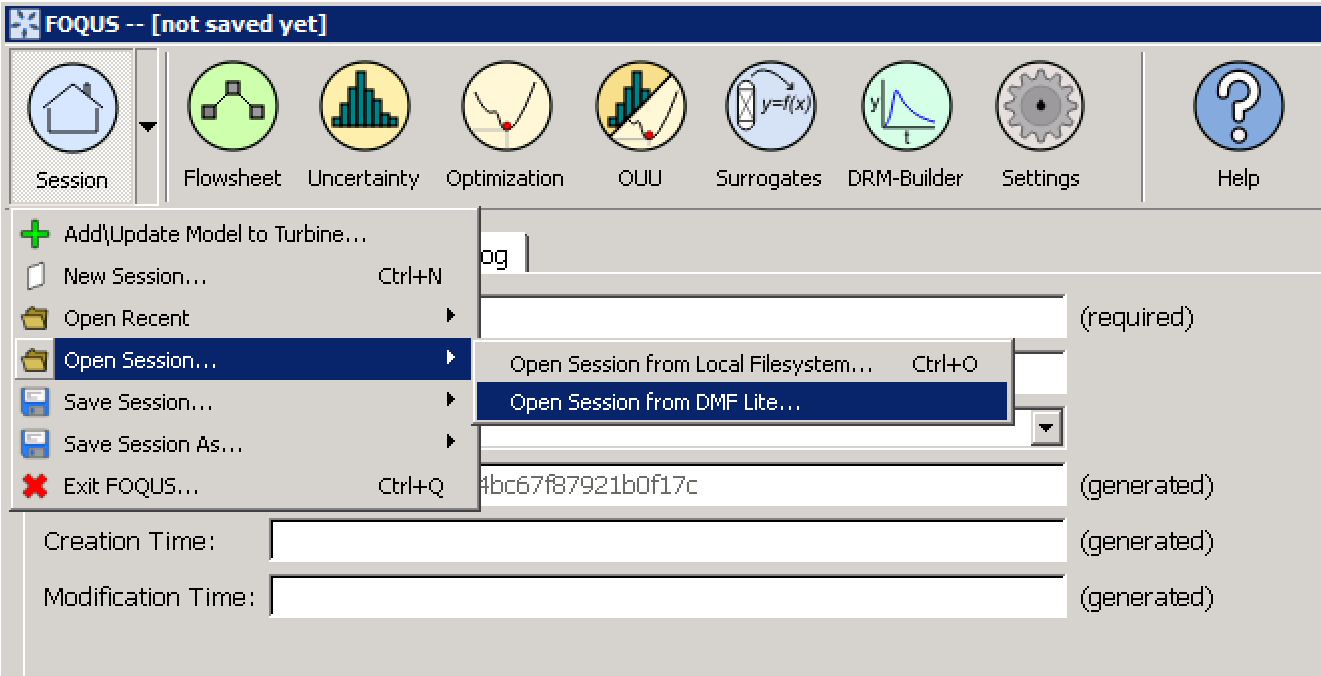
\includegraphics[width=.75\textwidth]{Chapt_flowsheet/figs/DMFFoqus}
  \caption{DMF-Related Submenus in FOQUS Session Menu}
  \label{fig:foqus-dmf-menu}
\end{figure}


If the property files and environment variables are setup correctly, menu items will display with
DMF-related submenus under the FOQUS \textbf{\underline{Session}} button (Figure~\ref{fig:foqus-dmf-menu}).
The subsequent subsections assume the correct setup of these property files and environment variables.

\subsection{Login Dialog (DMF with server)}
\label{login-dialog}

\begin{figure}[H]
  \centering
  \includegraphics[width=.5\textwidth]{Chapt_flowsheet/figs/login}
  \caption{DMF Login Prompt}
  \label{fig:login-dialog}
\end{figure}

This subsection is only relevant if using the DMF with a server. If the user is
planning to use only the DMF lite, skip this subsection.
When first connecting the DMF with a server, the user is prompted with a login dialog (Figure~\ref{fig:login-dialog}).
The user should login using the username and password given by the DMF server administrator
(instructions for creating these login credentials is provided at the DMF server side).

The user has the option of saving their user credentials so that they do not have to input their login credentials every time. To delete the saved
credentials, select {\textbf{\underline{Logout from DMF Repositories}} from the
\bu{Session} button drop-down menu, mentioned in Section~\ref{session-menu} (this option will display only when the DMF is enabled).
Logging out will remove all saved credentials from all repositories.

The login dialog feature is only relevant to the DMF lite when using the upload to server feature.

\subsection{Open Dialog}
\label{open-dialog}

The DMF open dialog (Figure~\ref{fig:open-dialog}) is accessible by selecting
\bu{Open Session} in the \bu{Session} button drop-down menu (Figure~\ref{fig:foqus-dmf-menu}),
mentioned in Section~\ref{session-menu}. This dialog enables the user to select and load a session file.
Associated simulation files are also opened with the intended session file.

\begin{figure}[H]
  \centering
  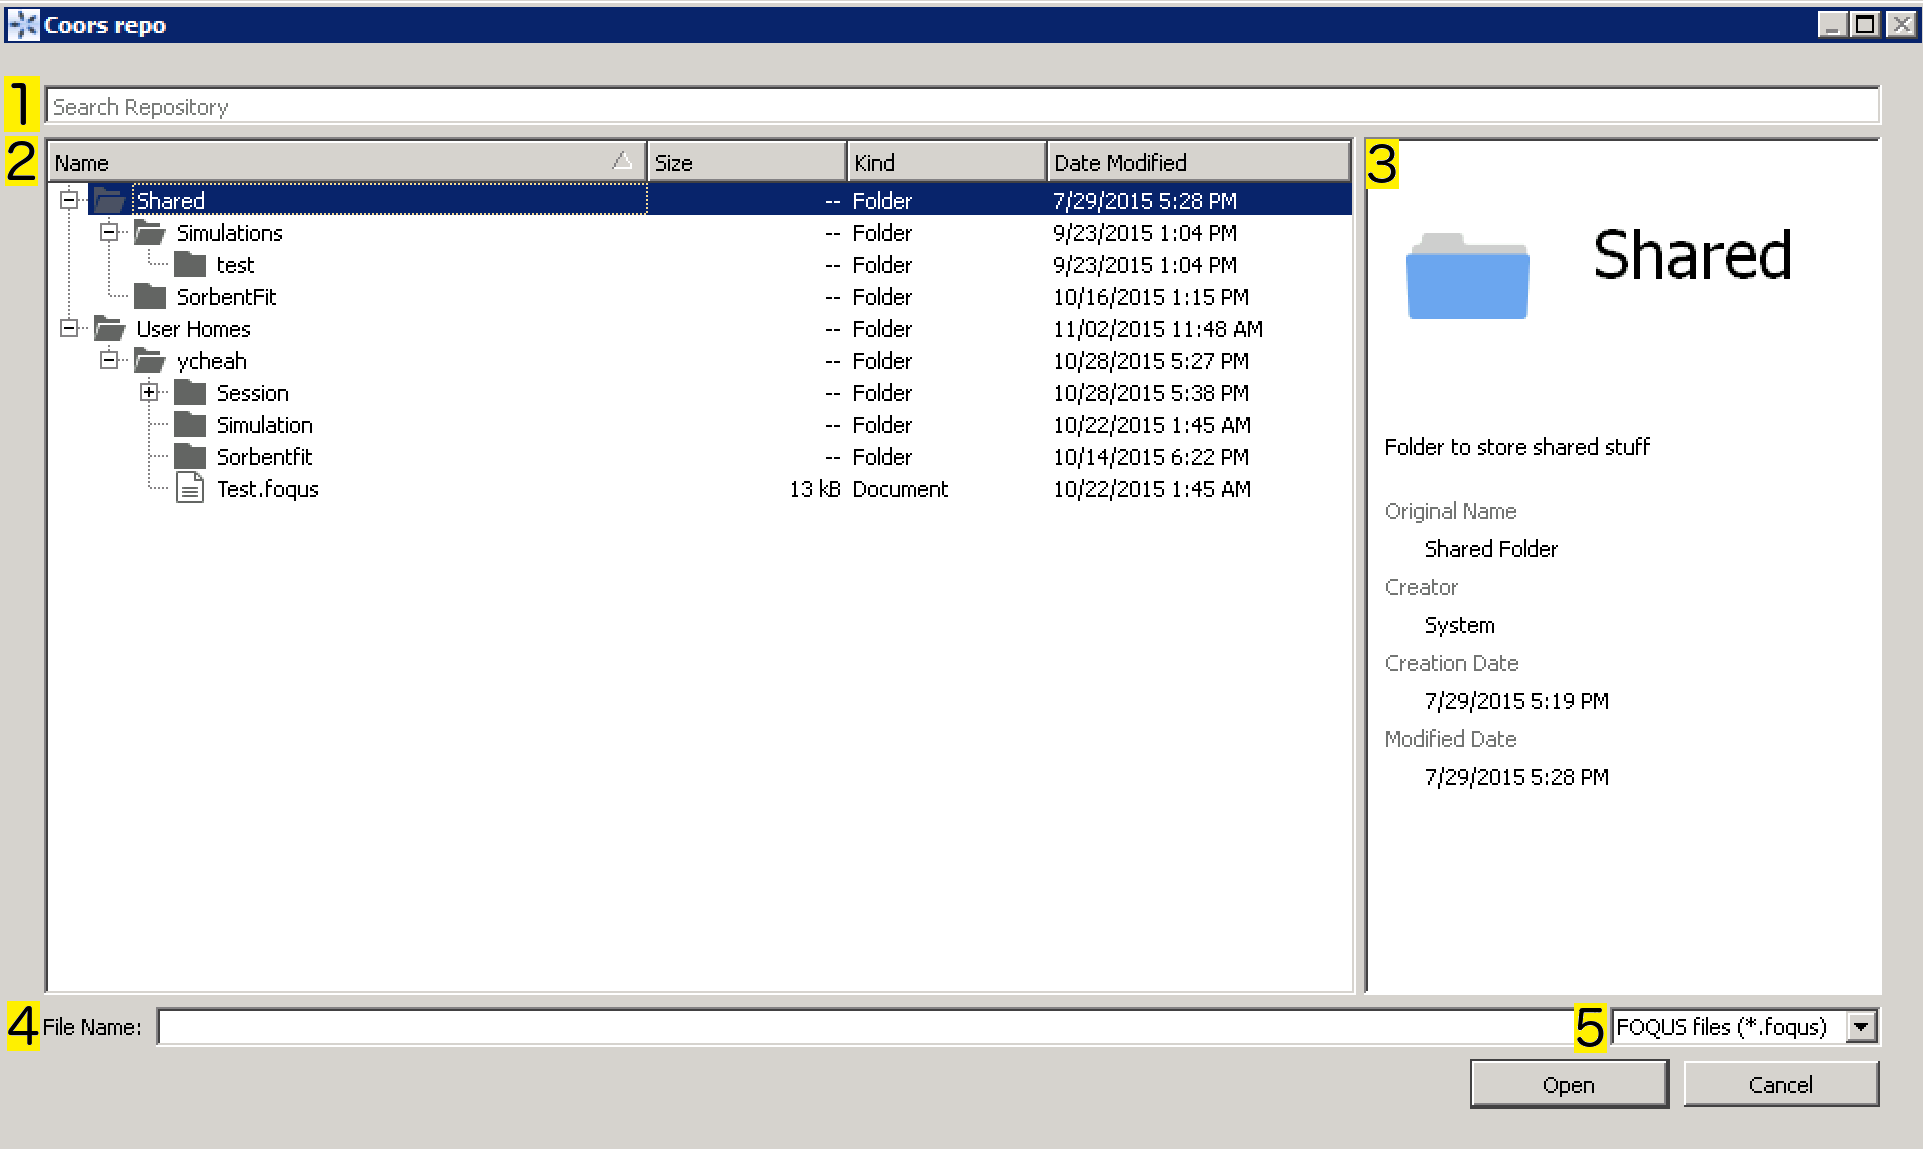
\includegraphics[width=.95\textwidth]{Chapt_flowsheet/figs/open-anno}
  \caption{DMF Open Dialog Box}
  \label{fig:open-dialog}
\end{figure}

\begin{enumerate}
\item \bu{Search Repository} for files. (This feature is not present in the DMF lite mode.)
  This text bar enables the user to search the repository. Some example queries are:
  \begin {enumerate}[label=(\alph*)]
  \item Search for items created on a specific date: created:``2014-09-22''
  \item Search for items modified between a date range: modified:``2014-09-22''..``2014-10-1''
  \item Search for items created by a certain username: creator:``ccsi''
  \item Search for items with a specific title: title:``session file''
  \item Wildcards can also be used. The following example is used to find all items with words starting with ``BFB*''.
  \item Conjunctions such as \textit{and} and \textit{or} can be used to chain queries
  \end {enumerate}

\item \bu{File Browser Pane} enables the user to navigate the DMF filesystem.
  Each user can view two root folders: (1) \textbf{\underline{Shared}} and (2) \textbf{\underline{User Homes}}. By default, each user can only view their home directory
  unless permissions are given to access additional directories at the DMF server side.
  When the search repository feature is used, the file browser displays matching files or folders of the query.
  (Note: By default, the pane is hidden but can be revealed by dragging the
  splitter at the right of the dialog box.)
\item \bu{Detailed Information Pane} provides detailed file metadata. By default, this is hidden. The pane can be opened by dragging the splitter at the right.
\item \bu{Selected File Name} displays the name of the selected file in the File Browser Pane.
\item \bu{File Display Filter} enables the user to filter based on the file types. The current implementation enables filtering of JSON files rather than viewing all files types.
\end{enumerate}

\subsection{Save Dialog}
\label{save-dialog}

\begin{figure}[H]
  \centering
  
\includegraphics[width=.95\textwidth]{Chapt_flowsheet/figs/save}
  \caption{DMF Save Dialog Box}
  \label{fig:save-dialog}
\end{figure}

The DMF save dialog (Figure~\ref{fig:save-dialog}) is similar to the open dialog and is accessible by selecting \bu{Save Session} in the \bu{Session} button drop-down menu
(Figure~\ref{fig:foqus-dmf-menu}, also discussed in Section~\ref{session-menu}). When a session is saved, associated simulation files are also ingested into the DMF.
The major differences between the ``open dialog'' and the ``save dialog'' are the \bu{Open} versus \bu{Save} buttons and the presence of a \bu{New Folder} button.

When \bu{New Folder} is clicked, the new folder dialog box (Figure~\ref{fig:new-folder}) displays.
There are three fields that require user input as follows:
\begin{enumerate}
\item \bu{Name} is the name of the folder and is a mandatory field, as indicated by the asterisk.
\item \bu{Description} is an optional field that enables the user to input the description of the new folder.
\item \bu{Fixed Form} accepts a true or false value: true indicates that the contents of the
folder cannot be altered; false indicates that the contents can be changed. The default for this
attribute is false (i.e., the contents can be changed).
\end{enumerate}

Similarly, when \bu{Save} is clicked, a dialog box (Figure~\ref{fig:new-file}) prompts the user to enter the session file metadata.
The following fields are associated with DMF files:
\begin{enumerate}
\item \bu{Display Name} is the name of the file and is the primary name stored in the DMF.
  This is a mandatory field as indicated by the asterisk.
\item \bu{Original File Name} is an optional field that can be used to indicate the original file name if different
  from what is saved in the DMF.
\item \bu{Description} is an optional field and enables the user to enter the description of the new file.
\item \bu{Mimetype} is a mandatory field for identifying the application that is meant to open this file.
\item \bu{External URL} is entered to specify the location of a file if stored at a remote location.
\item \bu{Version Requirements} is used to specify the version requirements of applications that use this file.
\item \bu{Confidence} specifies the stage of whether a file is experimental, at the testing stage, or the production stage. This defaults to experimental.
\end{enumerate}

\begin{figure}[H]
	\centering
	\centering
	\subfloat[New Folder dialog]{{\includegraphics[width=.25\linewidth]{Chapt_flowsheet/figs/folder-metadata}
			\label{fig:new-folder}}}%
	\qquad
	\subfloat[Save File Dialog]{{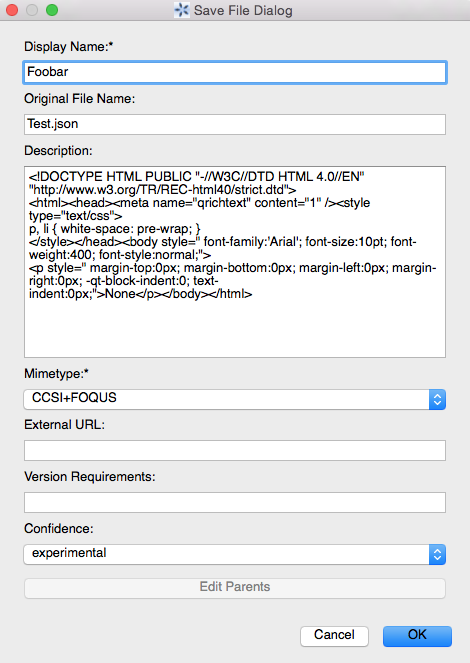
\includegraphics[width=.35\linewidth]{Chapt_flowsheet/figs/file-metadata}
			\label{fig:new-file}}}%
	\caption{Folder and File Metadata Input Dialog Box}
\end{figure}

\subsection{Browser}
The DMF Browser (Figure~\ref{fig:browser}) is a standalone tool that is bundled with the FOQUS toolsuite.
Although the browser shares the layout with the dialog boxes, there are a number of additional features.
It is meant to enable quick access to the data in the repository and view dependencies among files.
Instructions pertaining to property files and environment variables mentioned in Section~\ref{dmf-setup} are
also relevant to the use of the DMF Browser. The lite version of the DMF Browser (Figure~\ref{fig:lite-browser})
has a slightly different toolbar and
does not provide the functionality for dependency tracking.

\begin{figure}[H]
  \centering
  \includegraphics[width=.95\textwidth]{Chapt_flowsheet/figs/DMFBrowser}
  \caption{DMF Browser}
  \label{fig:browser}
\end{figure}

\begin{figure}[H]
  \centering
  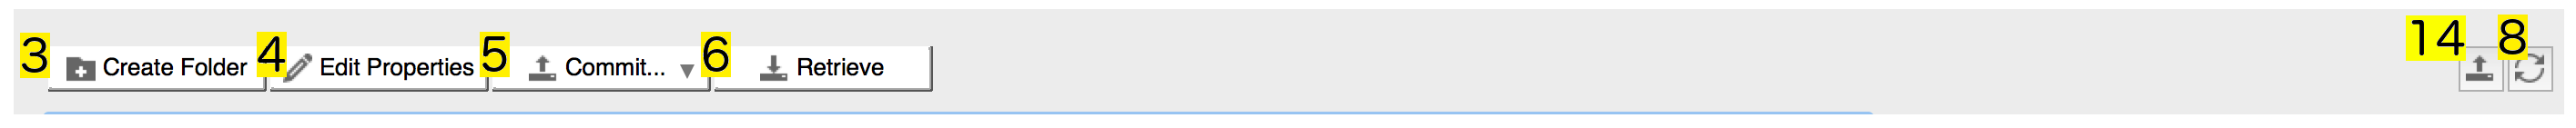
\includegraphics[width=.95\textwidth]{Chapt_flowsheet/figs/DMFLiteBrowser}
  \caption{DMF Browser Lite Toolbar}
  \label{fig:lite-browser}
\end{figure}

\begin{enumerate}
\item \bu{Search Repository} for files enables the user to search the repository. Example queries are as follows:
  \begin {enumerate}[label=(\alph*)]
  \item Search for items created on a specific date: created:``2014-09-22''
  \item Search for items modified between a date range: modified:``2014-09-22''..``2014-10-1''
  \item Search for items created by a certain username: creator:``ccsi''
  \item Search for items with a specific title: title:``session file''
  \item Wildcards can also be used. The following example is used to find all items with words starting with ``BFB*''.
  \item Conjunctions such as \textit{and} and \textit{or} can be used to chain queries.
  \end {enumerate}
\item \bu{Logout} allows the user to logout from the current session. The DMF browser will show a login prompt after logout.
\item \bu{Create Folder} allows the user to create a new folder in the desired parent folder. When the button is clicked,
  the new folder dialog box (Figure~\ref{fig:new-folder}) opens as discussed in Section~\ref{save-dialog}.
\item \bu{Edit Properties} displays menus that enable the user to edit file or folder metadata.
\item \bu{Upload/Commit} has two submenus: \bu{Upload File/Commit File} and \bu{Upload Folder /Commit Folder}
  that enables the user to upload files or folders from their local filesystem to the DMF Server.
  When uploading folders, the folder structure is maintained.
\item \bu{Download/Retrieve} enables the user to download the selected file or folder. In the case of a folder,
  a zip file of the folder and its contents are created when using the DMF Browser. When using the DMF Browser lite,
  a zip file is not created and the folder is simply created in the intended directory.
\item \bu{Lock} allows a file to be locked by a user. A locked file can no longer be overwritten and its properties cannot be edited.
\item \bu{Refresh} icon enables updating of the File Browser Pane.
\item \bu{File Browser Pane} enables the user to navigate the DMF filesystem.
  Each user can view two root folders: (1) \textbf{\underline{Shared}} and (2) \textbf{\underline{User Homes}}. By default, each user can only view their
  own home directory, unless permissions are given to access additional directories at the DMF server side.
  When the search repository feature is utilized, the file browser displays the matching files or folders of the query.
\item \bu{Detailed Information Pane} provides the detailed metadata of a file. The splitter in the \
  middle enables the pane to be resized as needed. In addition to what is available in the dialog boxes,
  a dependency graph of files is displayed when available.
\item \bu{Version} selector enables the user to navigate metadata associated with different versions of a file.
\item \bu{Undock Dependency Graph} enables the user to undock the dependency graph pane and view the dependencies in its own window.
\item \bu{Dependency Graph Pane} displays a dependency graph of the selected file in the File Browser Pane. The dependency graph
  always starts with the selected file and shows connections to ``ancestor'' files. The existence of these files are necessary and
  precede the generation of the selected file.
\item \bu{Upload to DMF Server} icon enables users to upload everything from the DMF lite to the DMF server. In order for this to work,
  the user must specify a .properties file for a DMF server. Other instructions pertaining to the use of the server based DMF in
  (Section~\ref{dmf-with-server}) will also need to be done prior to the use of this feature.
  The user will be prompted with a list of available DMF servers to log in.
  All files and folders are then created as a new version in the targeted DMF server in the user space.
\end{enumerate}

\subsection{Basic Data Model Ingest Tool}
\begin{figure}[H]
  \centering
  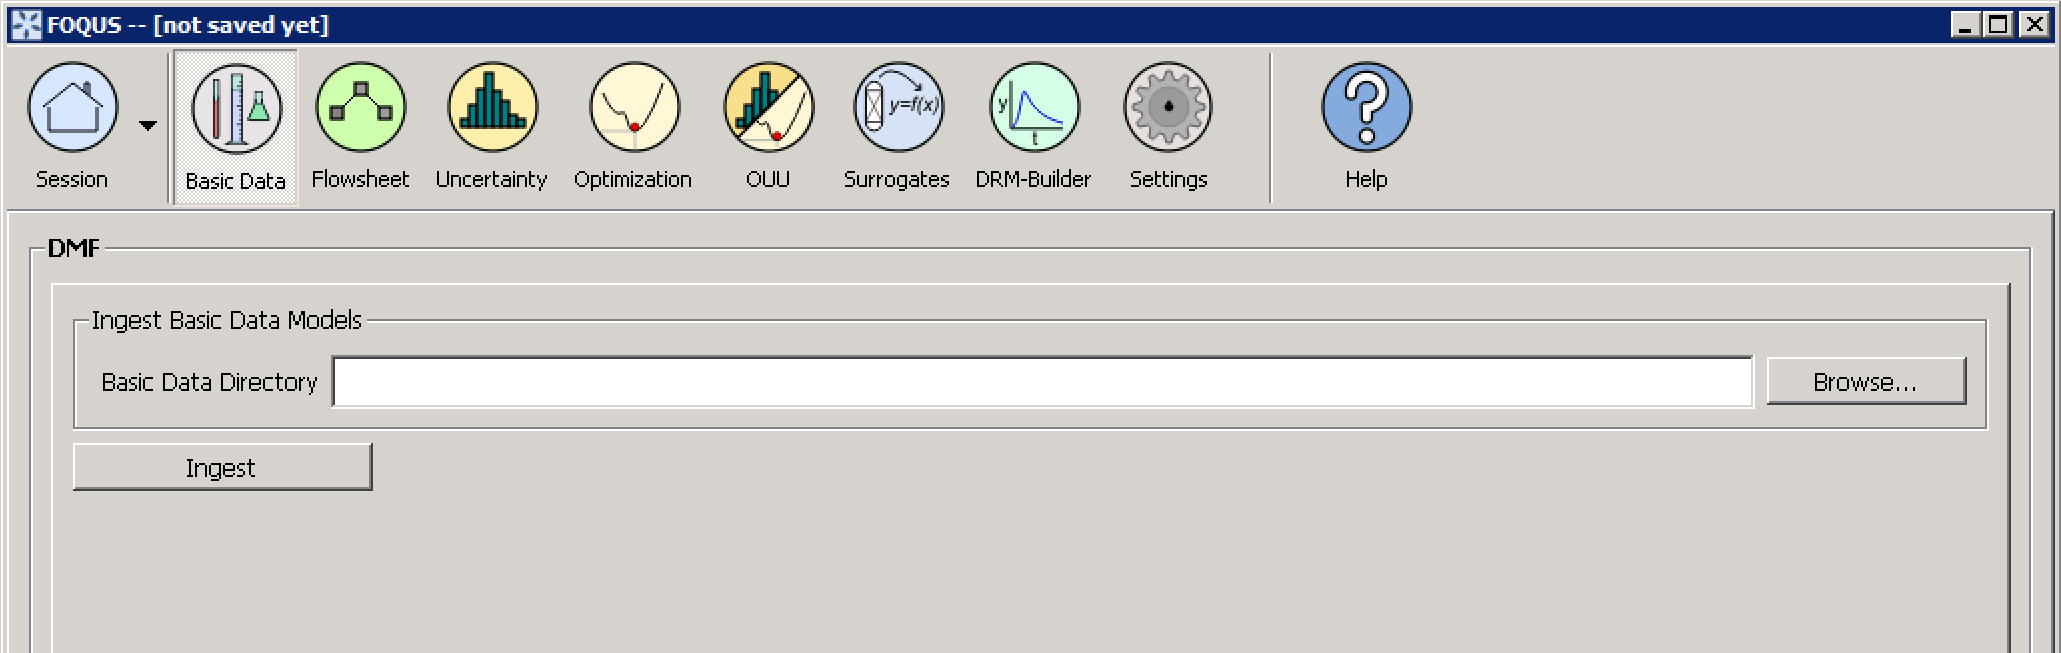
\includegraphics[width=.95\textwidth]{Chapt_flowsheet/figs/DMFBasicDataIngesterGUI}
  \caption{Basic Data Model ingester interface in FOQUS}
  \label{fig:basic-data-ingester}
\end{figure}


A simple command line script ingester is provided for use with basic data models. The tool can be
found under ``dmf\_lib/basic\_data'' in the FOQUS installation directory.
To launch the tool, run \textbf{python ingest.py} on the command line with arguments. A full list of potential arguments
will be printed on the command line when executed with the \textbf{-h} argument.

Alternatively, the tool can be launched from FOQUS via the Basic Data tab (Figure~\ref{fig:basic-data-ingester}).
By default, the Basic Data tab is hidden. When the \textbf{\underline{Use DMF if available}} checkbox (Figure~\ref{fig:foqus-dmf-settings})
is selected under the settings tab, and FOQUS is restarted, the Basic Data tab will be made available
(see Section~\ref{dmf-with-server} for detailed instructions).
Currently, the Basic Data Model ingest tool only supports ingesting basic data models into the server-based DMF.


\section{Tutorial -- Example Files}\label{tutorial.example.files}

Many of the tutorials in this manual make use of example files provided in the FOQUS installation.  This tutorial helps the user find and copy the example files.

\begin{enumerate}
	\item Locate the example files; they are in the FOQUS installation directory.  If the Windows installer was used, the files can usually be found in one of two locations:
	\begin{enumerate}
		\item 64-bit OS, C:\bs Program Files (x86)\bs foqus\bs foqus\bs examples
		\item 32-bit OS, C:\bs Program Files\bs foqus\bs foqus\bs examples
	\end{enumerate}
	\item Copy the example files directory to a convenient location for use in other tutorials.
\end{enumerate}
\section{Tutorial -- Creating a Flowsheet}\label{tutorial.simple.flow}

This tutorial provides information about the basic use of FOQUS and setting up a very simple flowsheet.  A single node flowsheet will be created that performs a simple calculation using a square root so that simulation errors can be observed when a negative input value is provided.

\begin{enumerate}
	\item Start FOQUS (see Section \ref{sec.flowsheet.starting.foqus}).
	\item In the session form enter the \textbf{\underline{Session Name}} as ``Simple\_Flow'' (Figure \ref{fig.session.name1}).
\end{enumerate}

\begin{figure}[H]
	\begin{center}
		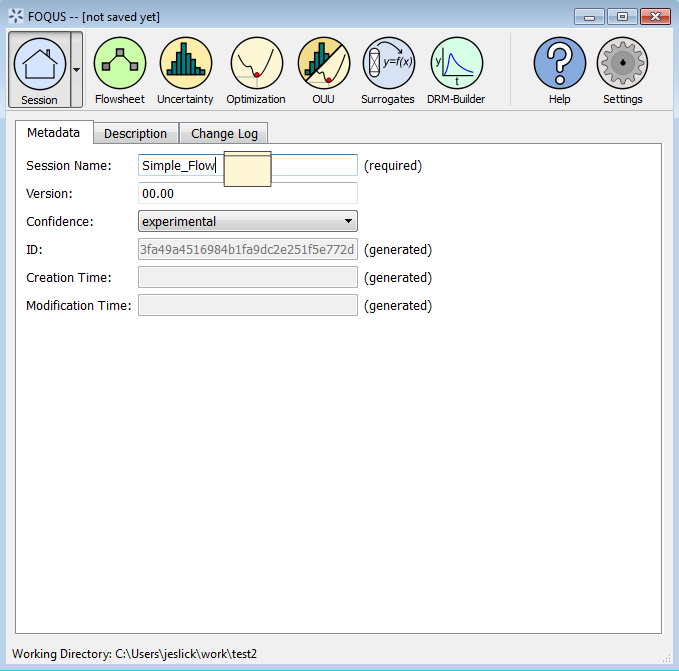
\includegraphics[scale=0.55]{Chapt_flowsheet/figs/session_name1}
		\caption{Setting the Session Name}
		\label{fig.session.name1}
	\end{center}
\end{figure}

\begin{enumerate}
	\setcounter{enumi}{2}
	\item Set the session description.
	\begin{enumerate}
		\item Select the \bu{Description} tab (Figure \ref{fig.session.description1}).
		\item Type the description shown in Figure \ref{fig.session.description1}.  The buttons above the \textbf{\underline{Description}} tab box can be used to format the text.
	\end{enumerate}
\end{enumerate}

\begin{figure}[H]
	\begin{center}
		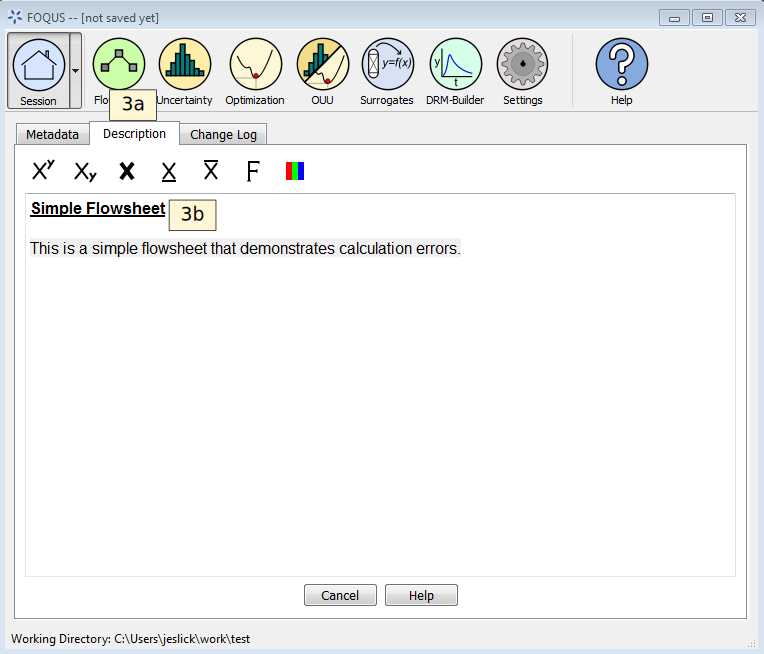
\includegraphics[scale=0.55]{Chapt_flowsheet/figs/session_description1}
		\caption{Setting the Session Description}
		\label{fig.session.description1}
	\end{center}
\end{figure}


\begin{enumerate}
	\setcounter{enumi}{3}
	\item Click the \textbf{\underline{Flowsheet}} button at the top of the Home window (Figure \ref{fig.simple.flow1}).
	\item Add a node named ``calc.''
	\begin{enumerate}
		\item Click the \textbf{\underline{Add Node}} button in the toolbar on the left side of the Home window.
		\item Click a location on the gridded flowsheet area.
		\item Enter the node name ``calc'' in the dialog box.
	\end{enumerate}
	\item Click the \textbf{\underline{Select Mode}} button in the toolbar.
	\item Open the Node Editor by clicking the \textbf{\underline{Node Editor}} button in the toolbar.
	\item Add input variables to the node. (When linking a node to an external simulation the input and output variables are populated automatically, and this step is not necessary.)
	\begin{enumerate}
		\item Click \bu{+} above the \textbf{\underline{Input Variables}} table.
		\item Enter x1 in the variable \textbf{\underline{Name}} dialog box.
		\item Click \bu{+} above the \textbf{\underline{Input Variables}} table.
		\item Enter x2 in the variable \textbf{\underline{Name}} dialog box.
		\item Enter -2 and 2 for the \textbf{\underline{Min}} and \textbf{\underline{Max}} of x1 in the \textbf{\underline{Input Variables}} table.
		\item Enter -1 and 4 for the \textbf{\underline{Min}} and \textbf{\underline{Max}} of x2 in the \textbf{\underline{Input Variables}} table.
		\item Enter 1 for the value of x1.
		\item Enter 4 for the value of x2.
	\end{enumerate}
\end{enumerate}

\begin{figure}[H]
	\begin{center}
		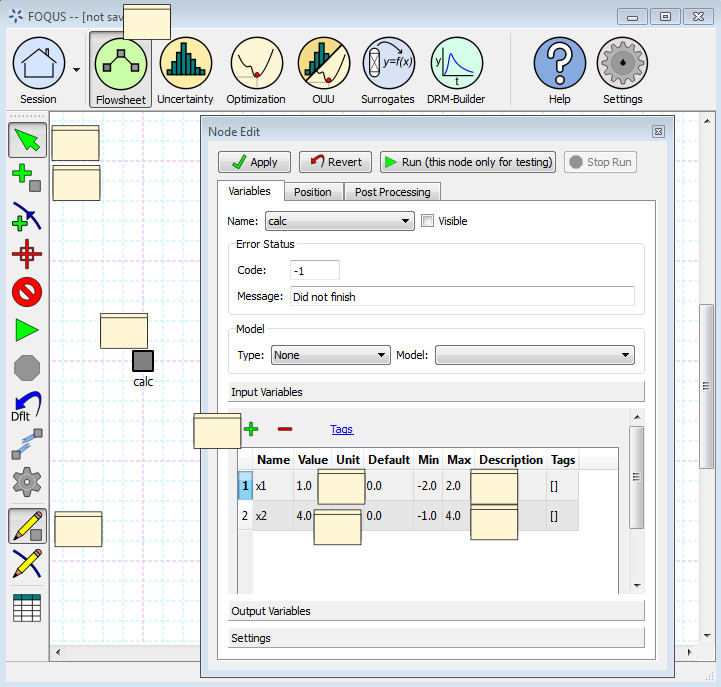
\includegraphics[scale=0.55]{Chapt_flowsheet/figs/simple_flow_1}
		\caption{Flowsheet, Input Variables}
		\label{fig.simple.flow1}
	\end{center}
\end{figure}

\begin{enumerate}
	\setcounter{enumi}{8}
	\item Add an output variable to the node. (When linking a node to an external simulation the input and output variables are populated automatically.)
	\begin{enumerate}
		\item Click \bu{Output Variables} to show the \textbf{\underline{Output Variables}} table (Figure \ref{fig.simple.flow2}).
		\item Click \bu{+} above the \textbf{\underline{Output Variables}} table to add a variable.
		\item Enter z in the output \textbf{\underline{Name}} dialog box.
	\end{enumerate}
\end{enumerate}

\begin{figure}[H]
	\begin{center}
		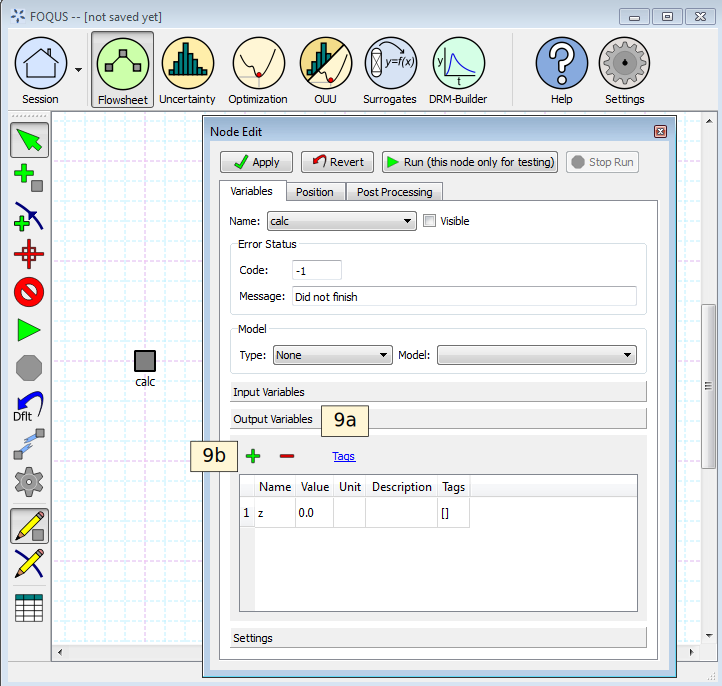
\includegraphics[scale=0.55]{Chapt_flowsheet/figs/simple_flow_2}
		\caption{Flowsheet, Output Variables}
		\label{fig.simple.flow2}
	\end{center}
\end{figure}

In this example, the node is not linked to any external simulation. The FOQUS nodes contain a section called node script, which can be used to do calculations before, after or instead of a simulation linked to the node. The node script can be used for things such as unit conversion, simple calculations, or simulation convergence procedures. The node scripts are written as Python. The \textbf{\underline{Input Variables}} are contained in a dictionary named x and the \textbf{\underline{Output Variables}} are contained in a dictionary named f. The dictionary keys are the variables names shown in the input and output tables. Only \textbf{\underline{Output Variables}} can be modified by a node script.

\begin{enumerate}
	\setcounter{enumi}{9}
	\item Add a calculation to the node.
	\begin{enumerate}
		\item Click the \bu{Node Script} tab (Figure \ref{fig.simple.flow3}).
		\item Enter the following code into the Python code box: \\ \verb|f['z'] = x['x1']*math.sqrt(x['x2'])|
	\end{enumerate}
	\item Click the \bu{Variables} tab.
	\item Click the \textbf{\underline{Run}} button (Figure \ref{fig.simple.flow3}).
\end{enumerate}

The flowsheet should run successfully and the output value should be 2. Rerun the flowsheet with a negative value for x2, and observe the result. The simulation should report an error.

\begin{figure}[H]
	\begin{center}
		\includegraphics[scale=0.55]{Chapt_flowsheet/figs/simple_flow_3}
		\caption{Node Calculation}
		\label{fig.simple.flow3}
	\end{center}
\end{figure}

\begin{enumerate}
	\setcounter{enumi}{9}
	\item Save the FOQUS session.
	\begin{enumerate}
		\item Click the \bu{Session} drop-down menu at the top of the Home window (Figure \ref{fig.simple.flow.save}).
		\item Click \bu{Save}. The exact location of save in the menu depends on whether or not the data management framework is enabled.
		\item The \textbf{\underline{Change Log}} entry can be left blank.
		\item The default file name is the session name. Change the file name and location if desired.
	\end{enumerate}
\end{enumerate}

\begin{figure}[H]
	\begin{center}
		\includegraphics[scale=0.55]{Chapt_flowsheet/figs/simple_flow_save}
		\caption{Save Session}
		\label{fig.simple.flow.save}
	\end{center}
\end{figure}



\section{Tutorial -- Creating a Flowsheet with Linked Simulations}\label{tutorial.sim.flowsheet}


This tutorial is referenced by other tutorials. \textbf{Save the flowsheet in a convenient location for future use.} 

This tutorial demonstrates how to link simulations to nodes, and how to connect nodes in a flowsheet.
Two models are used: (1) a bubbling fluidized bed model in ACM and (2) a cost of electricity (COE) model in Excel. The COE model estimates the cost of electricity for a 650 MW (net before adding capture) supercritical pulverized coal power plant with solid sorbent post combustion CO$_2$ capture process added.

Before starting the tutorial, see Section \ref{tutorial.example.files} to locate and copy the example files to a convenient location.

\begin{enumerate}
	\item Start FOQUS. The Session window displays (Figure \ref{fig.tut.opt.session}).
	\item Enter ``BFB\_opt'' in \bu{Session Name} (without quotes).
	\item Click the \bu{Description} tab. The problem description box displays and is shown in (Figure \ref{fig.tut.opt.description}).
	\item In the problem description box enter information about the problem being solved in the FOQUS session; this information can be more extensive than what is shown in the example.
	\item Save the session file. Click \textbf{\underline{Save Session}} from the \textbf{\underline{Session}} drop-down menu. Enter change log information and a file name when prompted. The \textbf{\underline{Creation Time}} in metadata page will be the time the session is first saved.  The \textbf{\underline{Modification Time}} will be the last time the session was saved. The \textbf{\underline{ID}} is a unique identifier that changes each time the user saves the simulation. The \textbf{\underline{Change Log}} tab provides a record of the changes made each time the session is saved.
\end{enumerate}

\begin{figure}[H]
	\begin{center}
		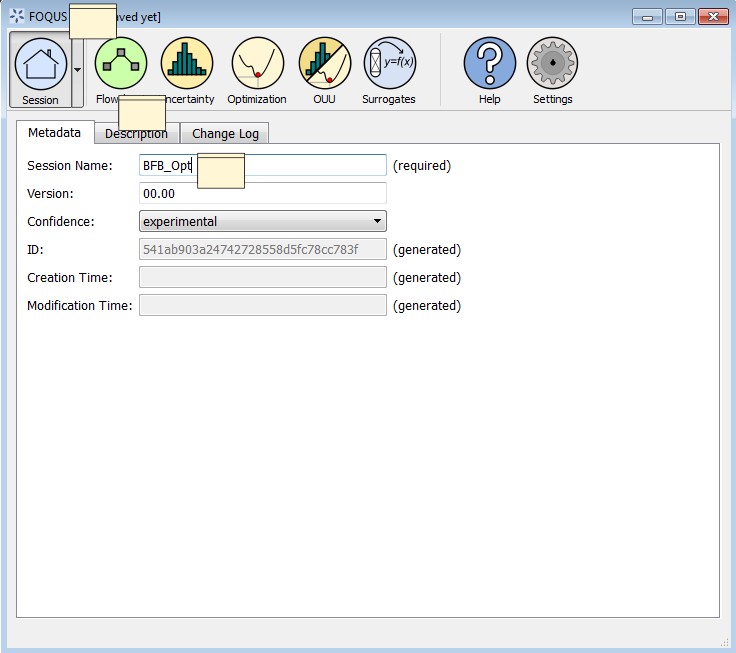
\includegraphics[scale=0.55]{Chapt_flowsheet/figs/session}
		\caption{Session Setup}
		\label{fig.tut.opt.session}
	\end{center}
\end{figure}

\begin{figure}[H]
	\begin{center}
		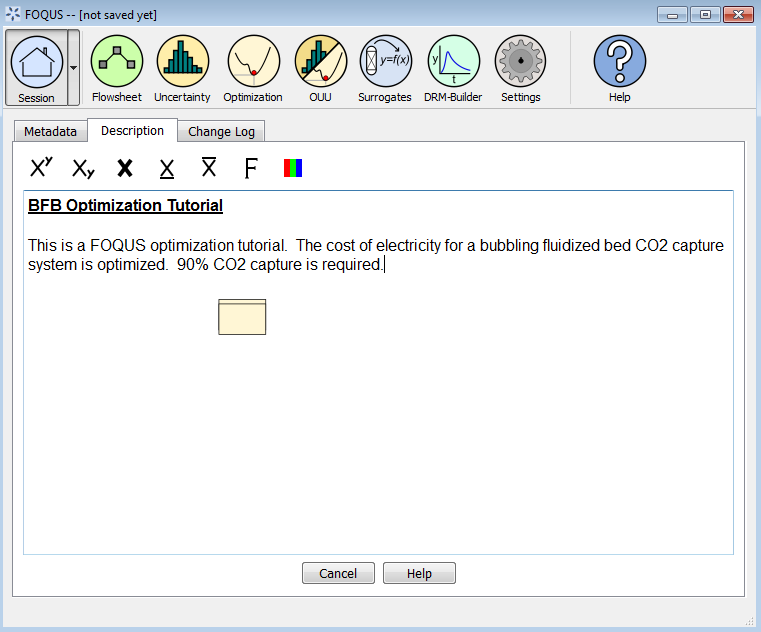
\includegraphics[scale=0.55]{Chapt_flowsheet/figs/description}
		\caption{Session Description}
		\label{fig.tut.opt.description}
	\end{center}
\end{figure}

\label{subsec.opt.tutorial.flowsheet}
There are two models needed for this optimization problem: (1) the ACM model for the BFB capture system and (2) the Excel cost estimating spreadsheet. These models are provided in the example files directory, under optimization/models (see Section \ref{tutorial.example.files}). There are two SimSinter configuration files: (1) BFB\_sinter\_config\_v6.2.json for the process model and (2) BFB\_cost\_v6.2.3.json for the cost model. The next step is to upload the models to Turbine.

\begin{enumerate}
	\setcounter{enumi}{5}
	\item Open the \bu{Add\bs Update Model to Turbine} dialog box (Figure \ref{fig.tut.opt.menu.upload}).
	\item In this case, the SimSinter configuration files have already been created. If a SimSinter configuration file needs to be created for the simulation, \bu{Create/Edit} displays the SimSinter configuration GUI (see Figure \ref{fig.tut.opt.upload}). See the SimSinter documentation or Chapter \ref{chapt.simsinter} for more information.
	\item Click \bu{Browse} to select a SimSinter configuration file (Figure \ref{fig.tut.opt.upload}). Once the SimSinter configuration file is selected, the simulation file and sinterconfig file is automatically added to the files to upload. The application type is entered automatically. If there are additional files required for the simulation, those files can be added by clicking \bu{Add File}.
	\item Enter the simulation name in \bu{Simulation Name}.  This name is determined by the user, but will default to the SimSinter configuration file name. For this tutorial use BFB\_v6\_2.
	\item Click OK to upload the simulation.
	\item Repeat the upload process for the cost model.  Name the model \\ BFB\_v6\_2\_Cost.
\end{enumerate}
\begin{figure}[H]
	\begin{center}
		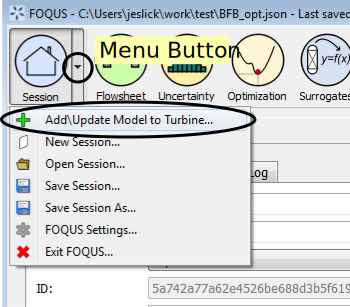
\includegraphics[scale=0.55]{Chapt_flowsheet/figs/menu_upload}
		\caption{Open Upload to Turbine Dialog}
		\label{fig.tut.opt.menu.upload}
	\end{center}
\end{figure}
\begin{figure}[H]
	\begin{center}
		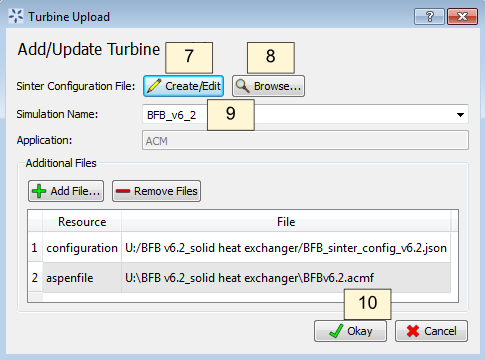
\includegraphics[scale=0.55]{Chapt_flowsheet/figs/upload}
		\caption{Upload to Turbine Dialog}
		\label{fig.tut.opt.upload}
	\end{center}
\end{figure}
The next step is to create the flowsheet.  Figure \ref{fig.tut.opt.drawFlowsheet} illustrates the steps to draw the flowsheet.
\begin{enumerate}
	\setcounter{enumi}{11}
	\item Click \bu{Flowsheet} at the top of the Home window.
	\item Click \bu{Add Node mode}.
	\item Add two nodes to the flowsheet. Name the first node ``BFB'' and the second node ``cost''.
	\item Click \bu{Add Edge mode}.
	\item Click the BFB node followed by the cost node.
	\item Click \bu{Selection mode} and select the BFB node.
	\item Click \bu{Toggle Node Editor}.  The Node Editor displays as illustrated in Figure \ref{fig.tut.opt.nodeEditor}.
\end{enumerate}
\begin{figure}[H]
	\begin{center}
		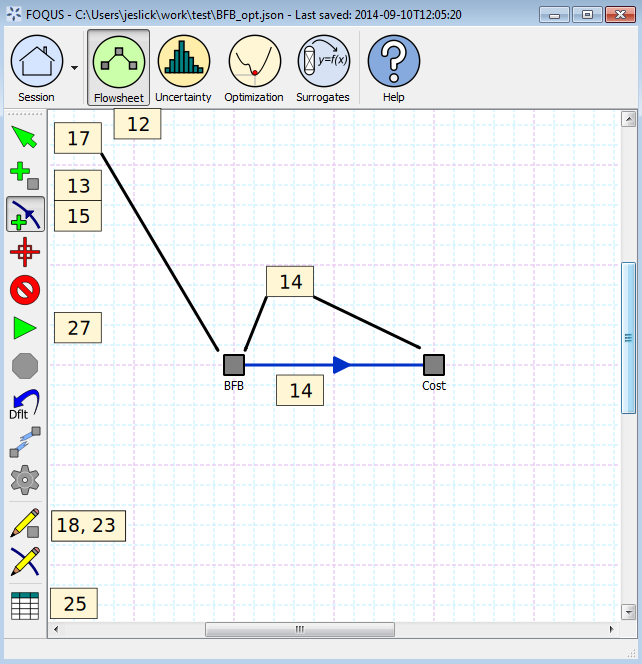
\includegraphics[scale=0.55]{Chapt_flowsheet/figs/flowsheetDraw}
		\caption{Flowsheet Editor}
		\label{fig.tut.opt.drawFlowsheet}
	\end{center}
\end{figure}
Each node must be assigned the appropriate simulation. Use the Node Editor to set the simulation type and the simulation name from simulation uploaded to Turbine. The Node Editor is illustrated in Figure \ref{fig.tut.opt.nodeEditor}
\begin{enumerate}
	\setcounter{enumi}{18}
	\item Under \bu{Model} and \bu{Type}, set the simulation \textbf{\underline{Type}} to Turbine. This indicates that the simulation is to be run with Turbine.
	\item Under \bu{Model}, set the simulation of the BFB node to BFB\_v6\_2.
	\item The \textbf{\underline{Variables}} and \textbf{\underline{Settings}} are automatically populated from the SimSinter configuration file. Variable values, \textbf\underline{{Min/Max}}, and descriptions can be changed; however, for this problem, the values taken from the SimSinter configuration should not be changed.
	\item Repeat the process for the cost node, assigning it the BFB\_v6\_2\_cost simulation.
\end{enumerate}
\begin{figure}[H] 
	\begin{center} 
		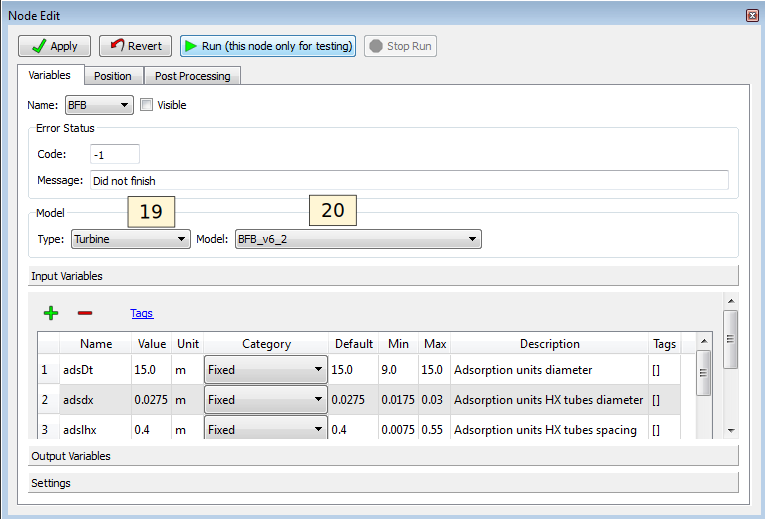
\includegraphics[scale=0.55]{Chapt_flowsheet/figs/nodeEditor}
		\caption{Node Editor}
		\label{fig.tut.opt.nodeEditor}
	\end{center}
\end{figure}
The connections between variables in the BFB simulation and the cost estimation spreadsheet must be set, so that required information can be transferred from the BFB simulation to the cost simulation.

\begin{enumerate}
	\setcounter{enumi}{22}
	\item Click \bu{Toggle Node Editor} to hide the Node Editor (Figure \ref{fig.tut.opt.drawFlowsheet}).
	\item Select the edge on the flowsheet with the \bu{Selection} tool.
	\item Click \bu{Toggle Edge Editor} to show the Edge Editor. The Edge Editor is shown in Figure \ref{fig.tut.opt.edgeEditor}.
	\item For convenience, all of the variables that should be connected from the ACM model to the Excel spreadsheet have been given the same names in their SimSinter configuration files. To connect the variables click \bu{Auto} in the Edge Editor.  \bu{Auto} connects variables of the same name. Since this is often not desired, the \bu{Auto} button should be used carefully. There should be 46 connected variables.
\end{enumerate}

\begin{figure}[H] 
	\begin{center} 
		\includegraphics[scale=0.55]{Chapt_flowsheet/figs/edgeEditor}
		\caption{Edge Editor}
		\label{fig.tut.opt.edgeEditor}
	\end{center}
\end{figure}

The flowsheet should now be ready to run. Test the flowsheet by executing a single evaluation before setting up the optimization problem.

\begin{enumerate}
	\setcounter{enumi}{26}
	\item Click \bu{Run} in the Flowsheet Editor (Figure \ref{fig.tut.opt.drawFlowsheet}).
	\item The flowsheet may take a few minutes to run.  The BFB simulation takes a significant amount of time to open in ACM. While running optimization, the evaluations take less time because the simulation remains opened. The simulation should complete successfully. A message box displays when the simulation is done. The status bar also indicates the simulation is running.
	\item While the simulation is running, \bu{Stop} is enabled.
	\item Once the simulation runs successfully, \textbf{\underline{Save}} the FOQUS session again, and \textbf{keep it for use in later tutorials}.
\end{enumerate}

\section{Tutorial -- Flowsheets with Recycle}

This section provides a tutorial on working with flowsheets containing recycle. Sections \ref{tutorial.simple.flow} and \ref{tutorial.sim.flowsheet} provide tutorials for creating flowsheets, in this section a pre-constructed flowsheet is used.

\begin{enumerate}
	\item From the example files, copy the Recycle\bs Mass\_Bal\_Test\_02.foqus example file to a convenient location (see Section \ref{tutorial.example.files}).
	\item Open FOQUS.
\end{enumerate}
\begin{samepage}\begin{enumerate}
	\setcounter{enumi}{2}
	\item Open the Mass\_Bal\_Test\_02.foqus file.
	\begin{enumerate}
		\item Open the \textbf{\underline{Session}} drop-down menu on the right side of the \textbf{\underline{Session}} button (Figure \ref{fig.recycle.tut1}).
		\item Select \bu{Open Session} from the drop-down menu.
		\item Locate Mass\_Bal\_Test\_02.foqus in the file browser, and open it.
	\end{enumerate}
	\setcounter{enumi}{3}
	\item Click \bu{Flowsheet} button from the toolbar at the top of the Home window.
\end{enumerate}\end{samepage}

The flowsheet is shown in Figure \ref{fig.recycle.tut1}.  The flowsheet consists of two reactors in recycle loops.  The flowsheet contains mixers, reactors, separators, and splitters. Each node uses a set of simple calculations in the node script section. The tear edges are shown in light blue.

\begin{figure}[H]
	\begin{center}
		\includegraphics[scale=0.55]{Chapt_flowsheet/figs/recycle_tut1}
		\caption{Flowsheet with Recycle}
		\label{fig.recycle.tut1}
	\end{center}
\end{figure}

\begin{enumerate}
	\setcounter{enumi}{4}
	\item Inspect a node.
	\begin{enumerate}
		\item Make sure the Selection tool is selected  (Figure \ref{fig.recycle.tut2}).
		\item Open the Node Editor by clicking the \textbf{\underline{Node Edit}} button in the left toolbar in the Flowsheet view.
		\item Click the ``React\_01'' node.
		\item Click \bu{Input Variables} table. Note: Some input rows are colored red. This denotes that their values are set by output of the previous flowsheet node by the edge connecting ``Mix\_01'' to ``React\_01.''
		\item Click the \bu{Node Script} tab.
		\item Note the equations. \textbf{\underline{Input Variables}} are stored in the x dictionary and \textbf{\underline{Output Variables}} are stored in the f dictionary.
	\end{enumerate}
	\item Click the gear icon in the left toolbar (see Figure \ref{fig.recycle.tut2}).  The tear solver settings are shown in Figure \ref{fig.tear.settings}.
\end{enumerate}
	
\begin{figure}[H]
	\begin{center}
		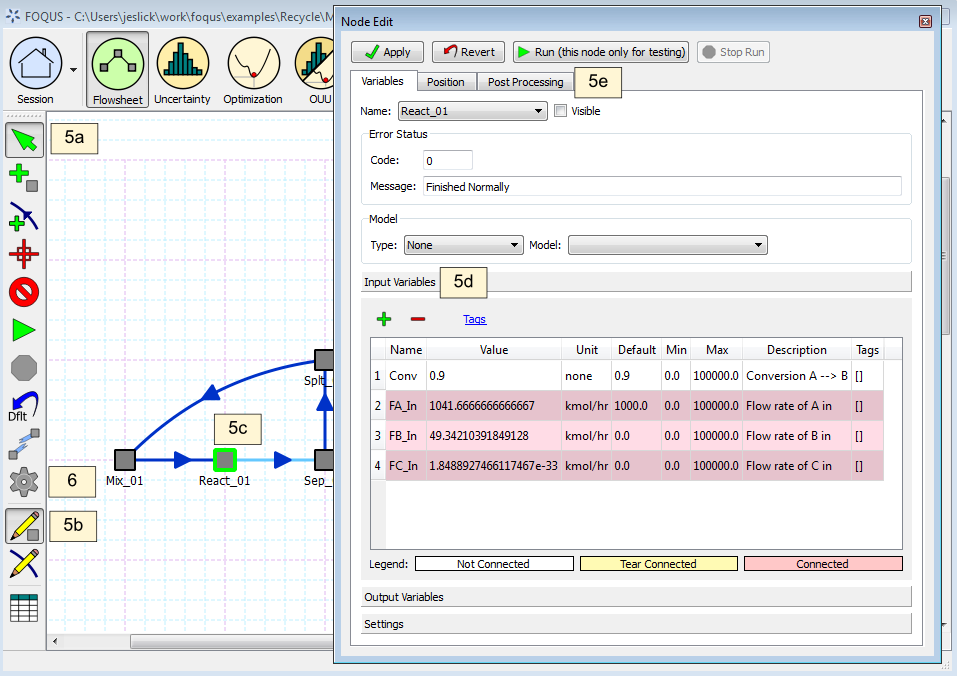
\includegraphics[scale=0.55]{Chapt_flowsheet/figs/recycle_tut2}
		\caption{React\_01 Node}
		\label{fig.recycle.tut2}
	\end{center}
\end{figure}

\begin{figure}[H]
	\begin{center}
		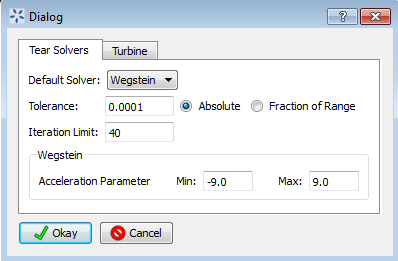
\includegraphics[scale=0.55]{Chapt_flowsheet/figs/tear_solver_settings}
		\caption{Tear Solver Settings}
		\label{fig.tear.settings}
	\end{center}
\end{figure}

\begin{samepage}
\begin{enumerate}
	\setcounter{enumi}{6}
	\item Remove the tear edges.
	\begin{enumerate}
		\item Close the Node Editor.
		\item Open the Edge Editor. Click the \bu{Edge Editor} icon in the left toolbar (see Figure \ref{fig.recycle.tut3}).
		\item Click the edge between ``React\_01'' and ``Sep\_01.''
		\item In the Edge Editor, clear the \bu{Tear} checkbox.
		\item Repeat for the other tear edge.
	\end{enumerate}
	\item Close the Edge Editor.
\end{enumerate}
\end{samepage}

\begin{figure}[H]
	\begin{center}
		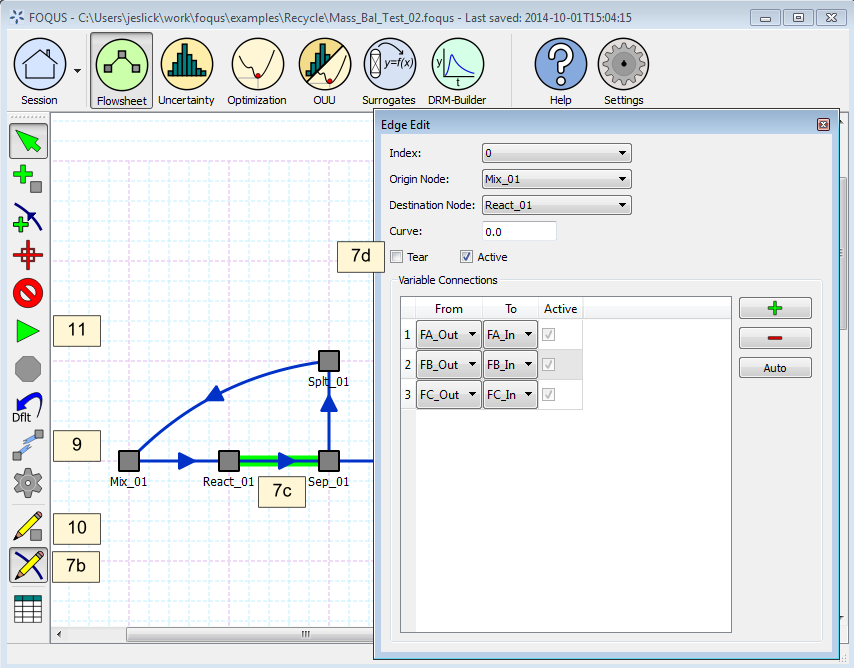
\includegraphics[scale=0.55]{Chapt_flowsheet/figs/recycle_tut3}
		\caption{Edge Edit}
		\label{fig.recycle.tut3}
	\end{center}
\end{figure}

There should now be no tear edges in the flowsheet. The user can select tear edges or FOQUS can automatically select a set. If there is not a valid set of tear edges marked when a flowsheet is run, tear edges will automatically be selected.
\begin{enumerate}
	\setcounter{enumi}{8}
	\item Automatically select a tear edge set by clicking the \bu{Tear} icon in the left toolbar (see Figure \ref{fig.recycle.tut3}).
	\item Open the Node Editor and look at node ``Sep\_01.''  In the Input Variables table, notice that some of the input lines are colored yellow. The yellow inputs serve as initial guesses for the tear solver. The final value will be different from the initial value.
	\item Click the \textbf{\underline{Run}} button on the left toolbar.  The flowsheet should solve quickly.
	\item The results of the completed run are in the flowsheet.  An entry will also be created in the Flowsheet Results data table (see Section \ref{tutorials.fs.data}).
\end{enumerate}


\subsection{Data Manipulation}

In this tutorial, instructions to change the data before analysis are
described. Current capabilities include sample filtering, input/output
variable deletion, and output value modification.

\subsubsection{Filtering}

Filtering involves selecting out samples whose values of a certain input or output fall into a certain range. Typically, when runs are returned from the Turbine gateway, there could be simulations that failed to converge in Aspen, thus the simulation samples corresponding to these failed runs should be excluded from analysis. Follow the steps below to filter out the samples due to failed runs:
\begin{enumerate}
	\item{Click \bu{Load from File} on the UQ window (Figure \ref{fig:uqt_data_filter}).}
	%%% INSERT: Data Manipulation, Filtering Tab
	\begin{figure}[H]
		\centering
		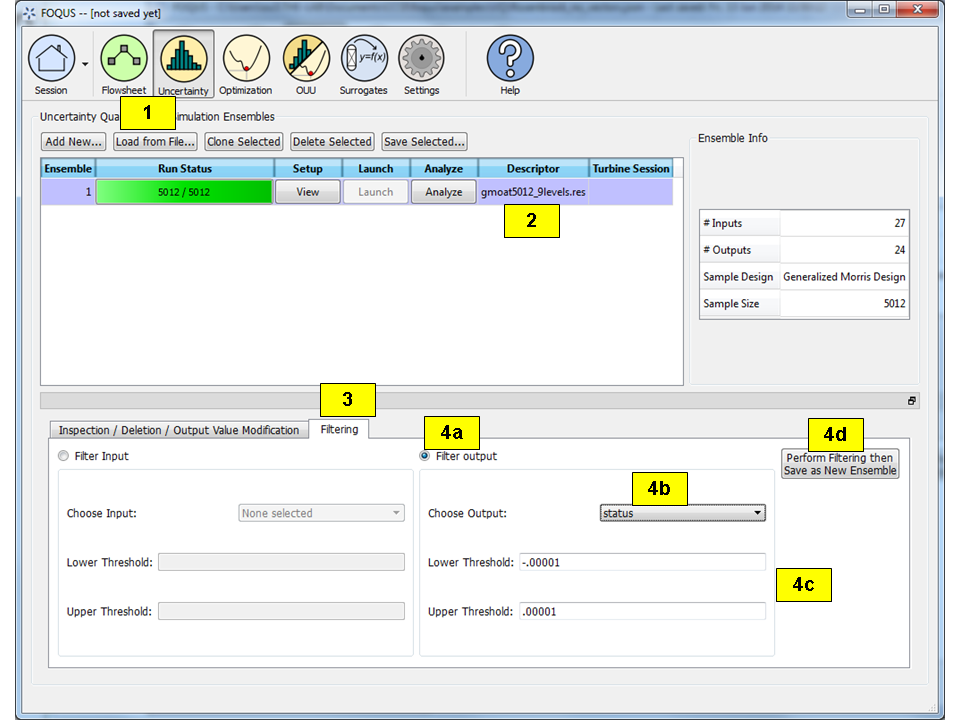
\includegraphics[width=6.5in,height=4in,keepaspectratio]{Chapt_uq/figs/tutorial/11_FilteringTab2}
		\caption{Data Manipulation, Filtering Tab}
		\label{fig:uqt_data_filter}
	\end{figure}
	\item{Select the file ``gmoat5012\_9levels.res'' in the examples\bs UQ folder. This
		file is an actual simulation ensemble that has already been run on the Turbine gateway.
		To find this file, the user may need to change the file filter to ``All files.''}
	\item{Select the \bu{Filtering} tab.}
	\item{Next, filtering the loaded simulation ensemble based on output values is performed. In particular,
		the user should keep only the samples in which the output parameter status is ``0.''}
	\begin{enumerate}
		\item{Select \textbf{\underline{Filter Output}}.}
		\item{Select ``status'' from the \textbf{\underline{Choose Output}} drop-down list.}
		\item{Enter -.00001 and .00001 as \textbf{\underline{Lower Threshold}} and \textbf{\underline{Upper Threshold}}
			respectively, and then click return within ``Lower threshold'' and ``Upper threshold.''}
		\item{Click \bu{Perform Filtering then Save as New Ensemble}.}
	\end{enumerate}
	\item{Once filtering is complete, a new row should be added to the
     simulation table (Figure \ref{fig:uqt_data_filter_results}). This
     ensemble contains only those samples that have a status value of
     ``0.'' Analysis can now be performed on this new ensemble because this
     ensemble contains only the valid simulations (i.e., those with output
     status value of 0), in which Aspen calculations have properly
     converged.
		%%% INSERT: Data Manipulation, Filtering Results
		\begin{figure}[H]
			\centering \includegraphics[width=6.5in,height=4in,keepaspectratio]{Chapt_uq/figs/tutorial/12_FilterResults2}
			\caption{Data Manipulation, Filtering Results}
			\label{fig:uqt_data_filter_results}
		\end{figure}
	}
\end{enumerate}

\subsubsection{Variable Deletion}
\label{subsubsec:uqt_vardel}

If an input or output variable is to be removed from consideration for
analysis, this can be done in the \bu{Inspection/Deletion/Output Value
  Modification} tab. Delete the status output from the previous filtering
as it is no longer needed for further analysis.
\begin{enumerate}
\item{Verify that the ensemble that resulted from filtering is selected. If not, select that ensemble.}
\item{Click the \bu{Inspection/Deletion/Output Modification} tab.}
\item{Scroll to the right of the table to the outputs, which are colored yellow.}
\item{Select the checkbox corresponding to the ``status'' output (the first output).}
\item{Click \bu{Perform Deletion then Save as New Ensemble}.}
\end{enumerate}
The results are illustrated in Figure \ref{fig:uqt_data_mod}. Note: The output count has decreased by one for the new ensemble. The user can verify that the ``status'' output was removed in the new ensemble by viewing this in the \textbf{\underline{Inspection/Deletion/Output Value Modification}} tab again. Deletion of an input can be performed similarly by selecting its checkbox and clicking the \textbf{\underline{Perform Deletion then Save as New Ensemble}} button.

%%% INSERT: Data Manipulation, Data / Output Value Modification Tab
\begin{figure}[H]
\centering 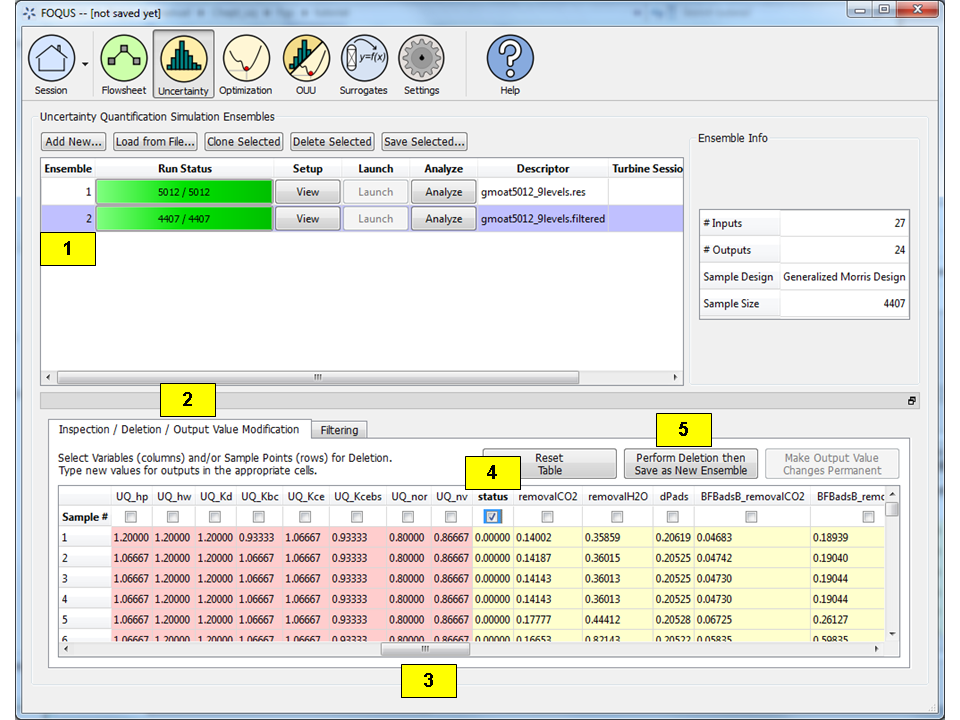
\includegraphics[width=6.5in,height=4in,keepaspectratio]{Chapt_uq/figs/tutorial/13_DataManipulation2}
\caption{Data Manipulation, Inspection/Deletion}
\label{fig:uqt_data_mod}
\end{figure}

\subsubsection{Output Value Modification}

To change the value of an output for a sample or several samples, follow steps below:
\begin{enumerate}
\item{Select an ensemble.}
\item{Click the \bu{Inspection/Deletion/Output Value Modification} tab.}
\item{Scroll to the right to the outputs.}
\item{Click on a cell for one of the outputs and enter a new value. Do the
  same for another cell. Notice that the modified cells turn green. This
  indicates the cells that have been modified.}
\item{Click \bu{Make Output Value Changes Permanent} to permanently change
  the values. The modified cells will turn yellow, indicating the permanent
  change. If the user wishes to reset the table and start over before
  making changes permanent, click the \bu{Reset Table}.}
\end{enumerate}

%%% INSERT: Data Manipulation, Output Value Modification
\begin{figure}[!htbp]
\centering \includegraphics[width=6.5in,height=4in,keepaspectratio]{Chapt_uq/figs/tutorial/14_DataManipulation_OutputModification2}
\caption{Data Manipulation, Value Modification}
\label{fig:uqt_data_mod_output}
\end{figure}

\pagebreak

\section{Tutorial -- Using a Remote Turbine Instance}\label{tutorial.fs.remote.turbine}

A remote Turbine instance may be used instead of TurbineLite. TurbineLite, used by default, runs simulations (e.g., Aspen Plus) on the user's local machine. The remote Turbine gateway has several potential advantages over TurbineLite, while the main disadvantage is the effort required for installation and configuration. Some reasons to run a remote Turbine instance are:
\begin{itemize}
	\item Simulations can be run in parallel.  The Turbine gateway can distribute simulations to multiple machines configured to run FOQUS flowsheet consumers.  FOQUS consumers are basically additional instances of FOQUS running on remote systems which can run a FOQUS flowsheet.
	\item Simulations can be run on machines other than the user's, so as not to tie-up the user's machine running simulations. 
\end{itemize}

The steps below demonstrate how to set up FOQUS to run flowsheets remotely (see Figure \ref{fig.remote.settings}).

\begin{enumerate}
\item Obtain a user name, password, and URL from the site's Turbine administrator.
\item Open FOQUS.
\item Click \bu{Settings} at the top right of the Home window (Figure \ref{fig.remote.settings1}).
\item Select ``Remote'' from the \bu{FOQUS Flowsheet Run Method} drop-down list. A message box will appear. The user will be warned that the models that have been uploaded to Turbine Local may not be available in Turbine Remote Gateway, which means that the user may need to upload the models into Turbine again (please see Step 7).
\item Click the \bu{Turbine} tab; this displays the Turbine settings shown in Figure \ref{fig.remote.settings}.
\end{enumerate}

\begin{figure}[H]
	\begin{center}
		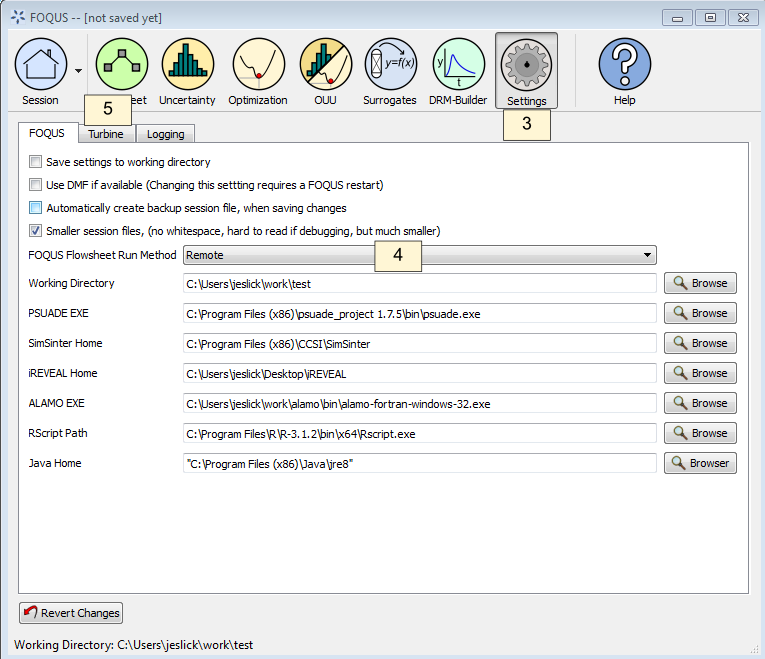
\includegraphics[scale=0.55]{Chapt_flowsheet/figs/settings_turbine_01}
		\caption{Run Method Settings}
		\label{fig.remote.settings1}
	\end{center}
\end{figure}

\begin{enumerate}
\setcounter{enumi}{5}
\item Create a Turbine configuration file; this contains your password in plain text, so it is very important that if you are allowed to choose your own password, you choose one that is not used for any other purpose.
\begin{enumerate}
	\item Click \bu{New/Edit} next to the \textbf{\underline{Turbine Configuration (remote)}} field. The Turbine Configuration window displays (see Figure \ref{fig.remote.settings}).
	\item Select ``Cluster/Cloud'' from the \bu{Turbine Gateway Version} drop-down list in the Turbine Configuration window.
	\item Enter the Turbine URL in the \textbf{\underline{Address}} field.
	\item Enter the \textbf{\underline{User}} name and \textbf{\underline{Password}}.
	\item Click \bu{Save as} and enter a new file name.
	\item Set the remote Turbine configuration file.  Click \bu{Browse} next to the \bu{Turbine Configuration (remote)} field. Select the file created in Step 6e.
\end{enumerate}
\end{enumerate}

\begin{figure}[H]
	\begin{center}
		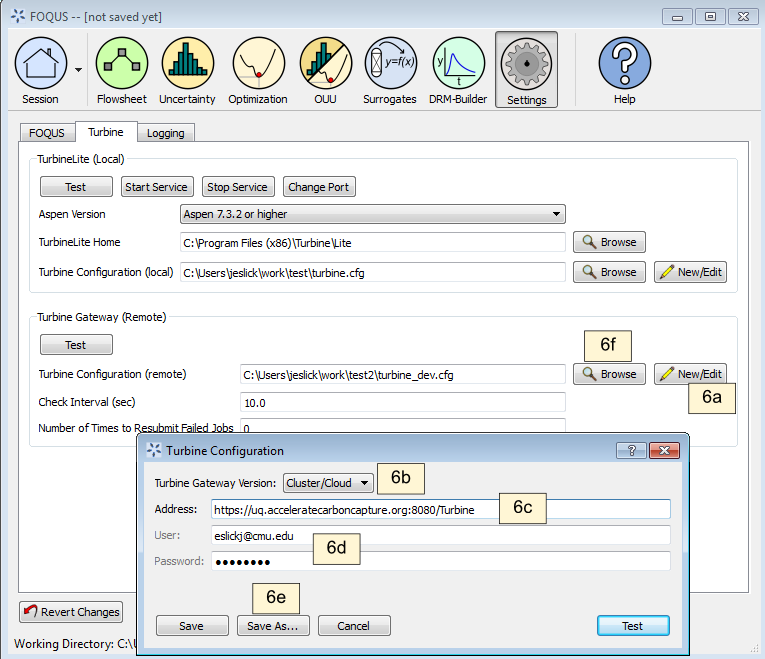
\includegraphics[scale=0.55]{Chapt_flowsheet/figs/remoteSetting}
		\caption{Remote Turbine Settings}
		\label{fig.remote.settings}
	\end{center}
\end{figure}

At this point the remote gateway is ready to use.  The last step is to ensure that all simulations referenced by flowsheets to be run are uploaded to the remote Turbine gateway.

\begin{enumerate}
	\setcounter{enumi}{6}
	\item Upload any necessary simulations to Turbine (see Section \ref{overview.turbine.upload} and the tutorial in Section \ref{tutorial.sim.flowsheet})
\end{enumerate}

Once all settings are specified there is no apparent difference between running flowsheets locally or on a remote Turbine gateway, and FOQUS can readily be switched between the two.

